\documentclass[12pt]{article}

%git add .
%git commit -m "modif"
%git pus

%----------------- PACKAGES -----------------

\newcommand{\citationpropre}[3]{
\vspace{1.7em}
\hrule
\vspace{0.8em}

\textit{#1}

\hfill \parencite[#2]{#3}

\vspace{0.6em}
\hrule
\vspace{1.7em}
}

\setlength{\skip\footins}{1cm}

\usepackage[T1]{fontenc}
\usepackage{newtxtext,newtxmath}
\usepackage[french]{babel}
\usepackage{csquotes}
\usepackage[a4paper, textwidth=16cm]{geometry}
\usepackage{graphicx}
\usepackage{titlesec}
\usepackage{changepage}
\usepackage{hyperref}

\addto\extrasfrench{
    \renewcommand{\figureautorefname}{Figure}
}

\usepackage{setspace}
\usepackage{xcolor}
\usepackage{fancyhdr}
\usepackage{chngcntr}
\usepackage{titlesec}

\setlength{\intextsep}{23pt}
\setlength{\textfloatsep}{20pt}
\usepackage{caption}
\captionsetup{skip=10pt}

\titleformat{\paragraph}
{\normalfont\normalsize\itshape}
{\theparagraph}
{1em}{}

\titlespacing*{\paragraph}{0pt}{6pt}{6pt}
%----------------- BIBLIOGRAPHIE APA -----------------
\usepackage[backend=biber,style=apa,language=french,maxcitenames=1,mincitenames=1]{biblatex}
\addbibresource{biblio.bib}
\DeclareLanguageMapping{french}{french-apa}
\DefineBibliographyStrings{french}{
  mathesis = {Mémoire de Master},
  phdthesis = {Thèse de Doctorat},
}
\newcommand{\filmcite}[1]{\textit{\citetitle{#1}} (\citeauthor{#1}, \citeyear{#1})}
%----------------- INTERLIGNE -----------------
\setstretch{1.5}

%----------------- NUMÉROTATION -----------------
\renewcommand{\contentsname}{Sommaire}
% Profondeur
\setcounter{secnumdepth}{4}
\setcounter{tocdepth}{4}

% Sections = I, II, III
\renewcommand{\thesection}{\Roman{section}}

% Sous-sections = 1, 2, 3 (SANS le I.)
\renewcommand{\thesubsection}{\arabic{subsection}}

% Sous-sous-sections = 1.1
\renewcommand{\thesubsubsection}{\arabic{subsection}.\arabic{subsubsection}}

\renewcommand{\theparagraph}{\thesubsubsection.\arabic{paragraph}}

%----------------- STYLE DES TITRES -----------------
\titleformat{\section}
  {\normalfont\large\bfseries}{\thesection}{1em}{}

\titleformat{\subsection}
  {\normalfont\normalsize\bfseries}{\thesubsection}{1em}{}

\titleformat{\subsubsection}
  {\normalfont\normalsize}{\thesubsubsection}{1em}{}

%----------------- HEADER / FOOTER -----------------
\setlength{\headheight}{14.5pt}

\pagestyle{fancy}
\fancyhf{}
\fancyhead[R]{\textcolor{gray}{\small Nohan Bresson}}
\fancyhead[L]{\textcolor{gray}{\small Synthétiser des ambiances naturelles pour le cinéma : l’exemple du vent}}
\fancyfoot[R]{\thepage}
\renewcommand{\headrulewidth}{0pt}

%----------------- INFOS DOCUMENT -----------------
\title{Utilisation de synthétiseurs d’ambiances naturelles dans la construction d’une bande son de film : l’exemple du vent}
\author{Nohan Bresson}
\date{2026}

\begin{document}

\begin{titlepage}
    \begin{center}
        % School Logo
        
\includegraphics[width=0.5\textwidth]{Images/logo LL.png} \\[1.5cm]

        % Thesis title
        {\LARGE \textbf{Utilisation de synthétiseurs d’ambiances naturelles dans la construction d’une bande son de film : l’exemple du vent}} \\[2cm]

        % Author
        {\large Nohan Bresson} \\[1cm]

        % Course
        {\large Mémoire de Master 2 - Spécialité Son} \\[1cm]

        % Supervisors / Directors
        {Directeur de mémoire :  Antoine Martin\\ 
        Référent et coordinateur mémoire : Corsin Vogel} \\[2cm]

        % Date
        {\large 2026}
    \end{center}
\end{titlepage}

\pagenumbering{roman}  % i, ii, iii, ...
\setcounter{page}{1}

\section*{Résumé}


\section*{Mots clés}



\newpage

\section*{Abstract}



\section*{Keywords}

\newpage

\section*{Remerciements}

\cleardoublepage           % Start on a fresh page (good for two-sided documents)

\tableofcontents

\cleardoublepage 
\pagenumbering{arabic}     % 1, 2, 3 ...
\setcounter{page}{1}       % Start at 1

\section*{Introduction}
\addcontentsline{toc}{section}{Introduction}
\leavevmode

Dans une grande partie des scènes de film (notamment en extérieur et dans la nature) si on souhaite une ambiance sonore cohérente avec l’image, le vent est une composante essentielle de la bande son. Il peut prendre de nombreuses formes (bourrasques, hululements, légères brises, simples fonds d’air...), se faire entendre sur différentes surfaces (bruissement de feuilles, d’herbes, de sable, “flap” de tissus...) et dans différents lieux (plaines, forêts, à travers une fenêtre...).

Dans la construction de la bande son, il est souvent pratique et utile d'utiliser des éléments sonores distincts et modulables. On peut alors traiter individuellement chacune des caractéristiques de ces sons (niveau sonore, timbre, dynamique, hauteur, spatialisation...). Or, il n’est pas toujours évident de trouver des ambiances adaptées à la scène et qui respectent ces contraintes. Ainsi, pourquoi ne pas recréer directement l’ambiance que l’on imagine ?

D’autre part, si on souhaite créer une ambiance de vent évolutive ou bien des effets (bourrasques, sifflements...) que l’on veut pouvoir contrôler (en temps, timbre, intensité, spatialisation...), l'utilisation d’un tel outil pourrait être un avantage. Pour une idée d’ambiance que l’on a, on peut faire l’hypothèse qu’utiliser un synthétiseur de ce type pourrait s’avérer plus efficace que de poser plusieurs couches sur notre montage son puis de faire varier leurs caractéristiques (volume, timbre, hauteur...). De même, des évènements ou effets ponctuels pourraient peut-être plus facilement être créés en jouant sur les contrôles du synthétiseur. Prenons l’exemple suivant : une scène dans laquelle le vent souffle en bourrasques sur un champ d’herbes hautes. Dans l’idéal, on aurait au minimum besoin de deux ambiances différentes du vent “pur” et des bruissements d’herbes. Ainsi, un synthétiseur pouvant contrôler simultanément l’intensité de ces deux ambiances pourrait s’avérer être un atout.

Reproduire le son du vent pour accompagner une histoire à laquelle un spectateur assiste est loin d’être une innovation. Dès le XVIIe siècle, des éoliphones (des machines à vent) étaient utilisés dans les concerts et les opéras. Des machines similaires ont également été utilisées un temps pour bruiter des dessins-animés ou des films. Des machines électroniques telles que le Windhowler ou le Windmaschine (maintenant émulées par Tonsturm) ont ensuite vu le jour au milieu du XXème siècle. Aujourd'hui, il existe également des synthétiseurs de bruitages ou d'ambiances naturelles (PANO de Noise Makers, rain de boom, Krotos Studio...) qui permettent de produire des sons variés (feu, eau, vent, bruitages...) modulables et souvent convaincants. Néanmoins, les possibilités de contrôle qu'offrent ces programmes ne permettent pas vraiment une construction d'ambiances évolutives et détaillées garantissant d'être en cohérence avec l'image du film.

\newpage

\section{État de l’art}

\subsection{Les sons environnementaux}

\subsubsection{Définition générale}

Tout d'abord, il est essentiel de définir ce qu'est une ambiance sonore. Pour cela, la notion de sons environnementaux au cinéma paraît pertinente à présenter. En voici une description accompagnée de quelques exemples : 

\citationpropre{Chaque lieu représenté dans une narration cinématographique contient des sons distincts et subtils provenant de son environnement. Ces sources sonores peuvent inclure, par exemple, le vent, la pluie, l'eau qui s'écoule, le bruissement des feuilles, le trafic lointain, les avions et les bruits de machines, les sons de mouvements et de paroles humaines à distance, les craquements dus aux variations thermiques, les climatiseurs et les installations de plomberie, le bruit des ventilateurs et des moteurs, le bourdonnement des machines électriques, le bruit de fond d'un espace, etc.\footnote{Every site depicted in a cinematic narrative contains distinct and subtle sounds emanating from its environment. These sound sources can include, for example, wind, rain, running water, rustling leaves, distant traffic, aircraft and machinery noise, the sound of distant human movement and speech, creaks and pops from thermal contraction, air conditioners and plumbing, the noise from fans and motors, the hum of electrical machines, room tone, etc.} }{p.~14}{chattopadhyay_auditory_2021}


Ici, deux caractéristiques importantes de ces sons sont abordées : ils représentent un environnement, un lieu, et s'inscrivent dans la narration du film. Les sources sonores données en exemple peuvent être humaines (voix, mouvements...), naturelles (pluie, vent...) ou anthropiques (machines, trafic...). 

D'après William W. Gaver\footnote{Co-directeur de l’Interaction Research Studio à la Northumbria University, et professeur au département de design de Goldsmiths, University of London}, une autre manière de qualifier ces sons environnementaux serait à partir des \enquote{phénomènes physiques des événements producteurs de son, abordés de manière qualitative}\footnote{[...] the physics of sound-producing events in a qualitative way} \parencite{gaver_what_1993}. Il propose ainsi une classification permettant de classer et décrire les sons de la vie de tous les jours, d'abord par trois catégories générales de matériaux, puis par les interractions qui peuvent leur permettre de produire du son (\autoref{fig:interacting_materials}).

\begin{figure}[ht]
    \centering
    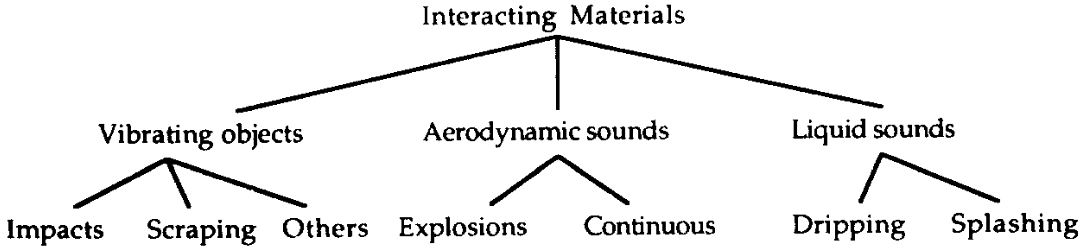
\includegraphics[width=0.7\textwidth]{Images/interacting_materials.png}
    \caption{Une description hiérarchique d'événements sonores simples \parencite[p.~22]{gaver_what_1993}}
    \label{fig:interacting_materials}
\end{figure}

Ce sont donc les caractéristiques des matériaux (structure, forme, densité...) et des phénomènes physiques qu'ils subissent (vitesse, puissance...) qui déterminent les caractéristiques acoustiques des sons produits. Gaver donne l'exemple du vent soufflant à travers un câble : la fréquence des vibrations produites va alors dépendre de la vitesse du vent, de la taille du câble et de sa tension \parencite{gaver_what_1993}.

Ainsi, décrire les sources sonores et l'environnement dans lesquelles elles existent permet de décrire de manière assez complète ce qui compose les sons environnementaux. Ces termes étant définis, on peut maintenant préciser le cadre de ce qui va nous intéresser pour ce mémoire, à savoir les ambiances naturelles. Pour cela, on s'appuiera principalement sur les notions suivantes.

\subsubsection{Paysages et écologie sonores}

Bernie Krause \footnote{Bernie Krause est un musicien, écrivain, maître de conférence et enregistreur de paysages sonores détenteur d'un doctorat en bioacoustique.} définit les paysages sonores ainsi :

\citationpropre{Le terme \textbf{paysage sonore} désigne tout environnement acoustique, qu'il provienne de sources naturelles, urbaines ou rurales. Il comprend l'ensemble des sons présents à un moment donné.\footnote{The term \textbf{soundscape} refers to any acoustic environment, whether it springs from natural, urban, or rural sources. It takes into account all of the sound present at any given time.}}{p.~22}{krause_wild_2002}

Ce terme s'inscrit dans le concept plus large d'\textit{écologie sonore} \footnote{acoustic ecology}, introduit par R. Murray Schafer et son assistant Barry Truax \footnote{Tous deux compositeurs, écrivains et enseignants.} à la fin des années 1970, c'est-à-dire \enquote{le champ d'étude qui s'intéresse aux relations entre les paysages sonores et les auditeurs, et à la manière dont la nature de ces relations caractérise la qualité d'un paysage sonore donné, qu'il soit urbain, rural ou naturel.} \footnote{[...] the field of study concerned with the relationships between soundscapes and listeners, and how the nature of these relationships characterize the quality of any given urban, rural, or natural soundscape.} \parencite{krause_wild_2002}. 

Ici, on s'intéressera principalement aux paysages sonores naturels. Krause les divise en deux catégories : la \textit{biophonie}, la \enquote{symphonie animale} et les paysages sonores composés des \enquote{sons que les organismes génèrent dans un habitat donné}, puis la \textit{géophonie}, qui regroupe ceux faits de \enquote{phénomènes non vivants, par exemple le bruit des ruisseaux, des tempêtes, du vent dans les arbres ou sur le sable, des éruptions et des tremblements de terre, ainsi que d'une multitude d'autres causes naturelles} \parencite{krause_wild_2002}.

Dans notre cas, c'est donc la géophonie qui va plus particulièrement nous intéresser. Une fois la nature de ces paysages sonores définie, il peut alors être intéressant de les décomposer et de préciser quels types de sons ils sont constitués.

\subsubsection{Texture sonore}

Pour \textcite{schwarz_state_2011}, la \textit{texture sonore} \footnote{\textit{sound texture}} est un composant essentiel et inhérent aux paysages sonores. Bien que \textcite{frojd_sound_2009} précisent qu'il n'y a pas de définition formelle et arrétée de ce qu'est une texture sonore, eux et les autres auteurs ayant travaillé sur ce sujet \parencite{strobl_sound_2006,schwarz_state_2011,athineos_sound_2003} s'accordent majoritairement sur les différentes caractéristiques données par \textcite{saint-arnaud_computational_1998} pour les reconnaître :

\citationpropre{(1) Les textures sonores sont constituées d'éléments sonores de base, ou « atomes » ; 
(2) ces atomes apparaissent selon un motif haut niveau, qui peut être périodique, aléatoire, ou les deux ; 
(3) les caractéristiques de haut niveau doivent rester stables sur de longues durées (ce qui implique l'absence de message complexe) ; 
(4) le motif de haut niveau doit être entièrement perceptible en quelques secondes (« durée d'attention ») ; 
(5) une part d'aléatoire à haut niveau est également acceptable, à condition qu'il y ait suffisamment d'occurrences dans cette durée d'attention pour constituer un bon exemple des propriétés aléatoires.
}{pp.~298--299}{saint-arnaud_computational_1998}

Ici, la « durée d'attention » désigne \enquote{le temps maximal entre des événements avant qu'ils ne soient perçus comme distincts. Quelques secondes constituent une durée d'attention raisonnable, mais, là encore, il n'existe pas de frontière nette} \parencite{saint-arnaud_computational_1998}. La durée du son ou plutôt le temps que l'on passe à l'écouter ainsi que la complexité des informations qu'il véhicule sont donc des points essentiels pour identifier une texture sonore. Le graphique de la \autoref{fig:sound textures in time} illustre bien cela : 

\begin{figure}[ht]
    \centering
    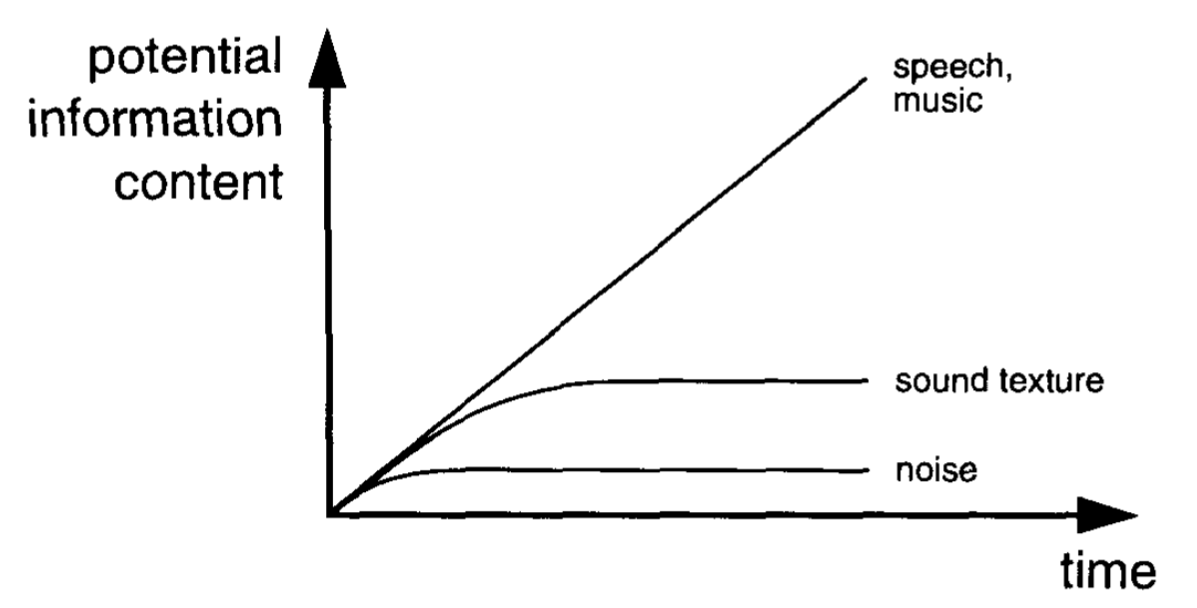
\includegraphics[width=0.65\textwidth]{Images/sound textures in time.png}
    \caption{Potentielles informations données par un son en fonction du temps d'écoute \parencite[p.~294]{saint-arnaud_computational_1998}}
    \label{fig:sound textures in time}
\end{figure}

Cette figure nous donne également des éléments afin de différencier un bruit \textit{(noise)} d'une texture sonore lors de l'écoute d'un son.

Maintenant que cette notion de texture sonore a été établie, on peut mieux expliquer les rapports qui existent entre elle et le paysage sonore. En effet, ce dernier est toujours composé en partie de textures sonores, mais en partie seulement, car il contient également des \enquote{sons ponctuels riches en informations} \parencite{schwarz_state_2011}. \textcite{schwarz_state_2011} donne également des exemples de textures sonores telles que la pluie, des foules, du vent tandis que \textcite{saint-arnaud_classification_1995} y ajoute le son d'une photocopieuse, des bulles dans un aquarium, une cascade, des vagues, des applaudissements, etc. On voit alors bien comment ces sons peuvent, dans certains contextes, ne représenter qu'un élément parmi d'autres d'un paysage sonore (par exemple une photocopieuse dans un bureau où des sonneries de téléphones retentissent) tandis que dans d'autres, ils peuvent en être l'unique composante (une grande cascade très bruyante). Ce mémoire s'inscrivant dans le cadre de la post-production son pour le cinéma, nous verrons dans le point suivant en quoi il est justement intéressant de pouvoir décomposer les paysages sonores en plusieurs éléments et comment les différentes ambiances sonores s'articulent lors de l'élaboration d'une bande son de film.


\subsection{L'ambiance sonore dans une bande son de film}
 \subsubsection{Définition, rôles et catégorisation}

Pour décrire largement l'ambiance sonore au cinéma, on peut tout d'abord s'appuyer sur cette première définition :

\citationpropre{L'ambiance sonore pourrait être décrite comme l'ensemble des sons qui constituent un arrière-plan sonore, presque un second plan, et construisent un environnement sur lequel peuvent s'appuyer les autres sons, ceux, plus saillants comme les voix, les bruits et les musiques, destinés plus principalement à la progression du récit. Les principales ambiances sont celles des sons de la nature (le vent, la mer, la forêt, la pluie...) et celles des activités humaines (foule, circulation, transports, sons industriels, parc, école, plage, gare...).}{}{adjiman_qualifier_2015}

La définition suivante proposée par \textcite{de_nanteuil_dictionnaire_2008} est également intéressante, permettant de donner un aperçu général de ce qui la caractérise, ainsi que du rôle qu'elle peut tenir :

\citationpropre{Dans la bande-son d'un film, l'ambiance sonore permet d'identifier ou de suggérer un lieu ou une situation (milieu urbain ou naturel, bruit de vent ou de foule, silence, etc.). Une ambiance sonore est généralement perçue de manière inconsciente comme une masse sonore globale et n'est pas nécessairement synchrone avec l'action qui se déroule à l'écran.}{}{de_nanteuil_dictionnaire_2008}

Dans ces deux descriptions, on retrouve plusieurs éléments importants tels que sa place dans le récit (importance narrative plus secondaire), son niveau sonore (plus bas que les autres éléments de la bande-son), la manière dont on la perçoit (« inconsciente », « masse sonore globale ») ou encore la fonction qu'elle peut occuper (« identifier ou [...] suggérer un lieu ou une situation », « construire un environnement »).

Leur intention narrative peut également être comprise par la notion de \textit{mise-en-sonore} introduite par \textcite{chattopadhyay_auditory_2021}. Elle \enquote{désigne un environnement sonore qui permet d'influencer la vraisemblance ou la crédibilité d'une œuvre cinématographique pour le spectateur} \footnote{[...] describe an auditory setting that in effect influences the verisimilitude or believability of a filmic work in the ears of its audience}. Elle permet également de faire ressentir une certaine sensation du lieu représenté à l'image, de donner une impression spécifique du décor filmé \parencite{chattopadhyay_auditory_2021}.

Les ambiances ont donc différentes fonctions possibles. \textcite{denizart_lemergence_2017} et \textcite{adjiman_qualifier_2015}, en s'appuyant notamment sur les travaux de de William Flageolet\footnote{Mixeur et ingénieur du son pour la musique au cinéma} et Michel Chion\footnote{Compositeur, théoricien et chercheur spécialisé dans les relations entre le son et l'image au cinéma.}, les classent en trois catégories :
\vspace{1em}

\begin{itemize}
    \setlength\itemsep{0.8em}
    \item \textbf{Les ambiances fonctionnelles} : elles établissent une continuité dans une séquence d'un film, permettant à l'image la liberté de changer de plan, d'axe, de point, etc. Les fonds d'air en sont un bon exemple : ils n'ont que peu d'apports sur la narration mais forment une sorte de liant entre les différents plans d'une même séquence, comblent le vide sonore et couvrent les éventuels changements de bruits de fond du son direct pris sur le tournage entre les différentes prises. Leur intérêt est donc avant tout pratique et technique.
    \item \textbf{Les ambiances territoires} : elles se basent une sur une description causale du son, \enquote{c'est-à-dire une description qui s'en tienne exclusivement à l'origine acoustique de la production du son} \parencite{adjiman_qualifier_2015}. Elles illustrent par le son les environnements et les éléments présents à l'écran ou que l'on peut imaginer existants en hors-champ.
    \item \textbf{Les ambiances narratives} : elles transmettent des intentions artistiques, émotionnelles ou symboliques sur la narration, le ressenti des personnages, une interprétation ou une sensation que le réalisateur veut transmettre à l'audience. Elles peuvent tenir un rôle qui se rapproche de celui d'une musique en apportant par exemple au récit \enquote{du rythme, de la tension ou une impression de douceur} \parencite{adjiman_qualifier_2015}. Enfin, elles ne sont pas nécessairement employées dans une volonté de maintenir une cohérence avec l'image.
\end{itemize}
\vspace{1em}

On peut rajouter que ces catégories ne sont pas nécessairement excluantes entre elles, une même ambiance pouvant entrer dans plusieurs de ces catégories ou évoluer d'une catégorie à une autre au cours d'une scène. Les caractéristiques des ambiances sonores dans les définitions données précédemment sont elles aussi à prendre à titre indicatif général. Par exemple, bien qu'elles puissent souvent être perçues inconsciemment, elles ne sont pas systématiquement reléguées au second plan, aussi bien en terme de niveau sonore que d'importance dans la narration. \textcite{adjiman_usages_2018} donne l'exemple de la séquence du duel final dans \filmcite{il_buono_il_brutto_il_cattivo_1966}\footnote{\textit{Le Bon, la Brute et le Truand}}. Ici, des ambiances telles que le soufle du vent et les sons de la faune du désert ont une fonction essentielle dans la narration, participant à renforcer la tension qui s'installe dans la scène. Ces sons sont alors \enquote{au même niveau sonore élevé où pourraient se situer une musique ou des bruits discrets} \parencite{adjiman_usages_2018}.

Détailler les autres types de sons qui constituent, avec les ambiances, la bande-son d'un film peut également être intéressant pour mieux scerner ces dernières et observer ici encore l'existance d'une certaine perméabilité entre ces catégories. En s'appuyant sur les travaux de \textcite{balibar2015chaine}, \textcite{denizart_lemergence_2017} en propose trois autres en plus des ambiances, accompagnées des traits pertinents qui les caractérisent :
\vspace{1em}

\begin{itemize}
    \setlength\itemsep{0.8em}
    \item \textbf{La matière phonique} : production de l'acteur, langue naturelle parlée.
    \item \textbf{La matière musicale} : production du compositeur, harmonicité, rythmicité.
    \item \textbf{Les bruitages et les effets} : production du bruiteur ou du monteur son, bref, ponctuel, saillant.
\end{itemize}
\vspace{1em}

En précisant notamment quel corps de métier a généralement la responsabilité de créer chacun de ces sons et donc à quel moment de la production ou post-production du film on les élabore, on a alors une nouvelle approche pour classer les sons qui peuvent être ambigus (une nappe sonore peut avoir un aspect musical mais être produite par le monteur son, un bruitage continu comme un bruissement de feuilles pourrait être assimilé à ambiance...).

Ainsi, l'étape pendant laquelle les ambiances sonores vont principalement être créées, choisies et intégrées à la bande-son d'un film est celle du montage son.

\subsubsection{Le montage son des ambiances}

De manière globale, cette phase de de la post-production sonore d'un film (qui intervient après le montage image et avant le mixage) est de nos jours assurée par un, une ou plusieurs monteurs et monteuses son. Contrairement aux métiers de chef opérateur son \footnote{Le chef opérateur du son (également appelé, « ingénieur du son ») et le perchman  enregistrent sur le tournage les voix des comédiens, les sons synchrones à l'image  et divers sons seuls \parencite{denizart_lemergence_2017}} et de mixeur \footnote{Le mixeur équilibre les sons et finalise la bande sonore \parencite{denizart_lemergence_2017}} qui naissent pratiquement avec la naissance du cinéma parlant, celui-ci son apparaît plus récemment, au début des années 1980 \parencite{denizart_lemergence_2017}. Pour les ambiances, \enquote{en France, le travail de cette matière sonore mobilise systématiquement un technicien spécifique : le monteur son des ambiances et des effets (qui travaille en coopération avec le monteur son des sons directs et des paroles)} \parencite{adjiman_usages_2018}. C'est à ce stade que \enquote{le monteur son "ajuste, propose, suggère les éléments sonores qui contribueront  au récit et à l'émotion des spectateurs". Il choisit des sons additionnels, organise la matière sonore et construit la bande-son} \parencite{denizart_lemergence_2017}. Il va également \enquote{contribuer à la construction des espaces sonores, s’occuper des  événements synchrones à l’image et prolonger le travail narratif déjà entrepris lors  du montage image} \parencite{denizart_lemergence_2017}.

\leavevmode

L'ambiance sonore que l'on commence à créer durant cette étape est en fait quasi systématiquement composée de plusieurs sources différentes, et ce pour plusieurs raisons, \enquote{que ce soit pour laisser la possibilité d'intervenir de manière individuelle sur chaque son, de les disposer différemment dans l'espace multicanal ou finalement de ne pas en retenir certains pendant le mixage} \parencite{adjiman_pour_2015}. C'est pourquoi on fonctionne avec \enquote{une logique de "couches", c'est-à-dire à travers une méthode qui enjoint à discriminer chaque événement sonore en autant de pistes superposées de son logiciel de montage} \parencite{adjiman_pour_2015}. En procédant ainsi, on peut donc construire des ambiances complexes et évolutives, comprenant plusieurs sons différents qui peuvent êtres ajustés, modifiés et spatialisés individuellement durant le montage son et le mixage.

Si on prend par exemple une séquence de film durant laquelle on veut créer une ambiance territoire (définie précédemment), la prise de son directe d'une ambiance sur le lieu de tournage pendant les prises ou en sons seuls ne représentera pas forcément fidèlement l'environnement que l'on souhaite faire entendre et resentir au spectateur. On sera alors amené à créer des couches d' \enquote{enregistrements audio mettant en scène peu de sons différents ou du moins peu de sons simultanés} \parencite{adjiman_pour_2015} pour créer l'ambiance finale complexe et modulable que l'on souhaite, une \enquote{entité cohérente et crédible} \parencite{adjiman_pour_2015}

Mais ce fonctionnement par couches n'a pas forcément et seulement comme fonction de tendre vers une représentation sonore réaliste et cohérente de l'environnement filmé. De manière plus générale, afin de représenter un lieu ou une atmosphère, les enjeux du travail de construction des ambiances sonores dans une bande-son de film pourraient se résumer ainsi : 

\citationpropre{Les choix esthétiques qui déterminent la qualité, le volume, la texture, la conception et la spatialisation de ces couches sonores d'ambiance influencent la présence de lieux spécifiques dans le monde diégétique du film.\footnote{Aesthetic choices that determine the quality, volume, texture, design and spatialisation of these ambient sound layers will impact the presence of specific sites in the cinematic story-world} }{p.~36}{chattopadhyay_auditory_2021}

\leavevmode

Plus globalement,  l'ambiance elle-même a pris de plus en plus en plus d'importance et de temps de travail dans la création sonore à l'image au fur et à mesure des évolutions technologiques que le son pour le cinéma a connu depuis 100 ans.

On peut tout d'abord observer cela avec la généralisation du son multicanal dans les films et les cinémas. Aujourd'hui, le montage son pour le cinéma se fait essentiellement sur et pour des systèmes de diffusion multicanaux. Dans ce contexte là, on pourrait définir le son multicanal comme suit :

\citationpropre{Système de reproduction sonore comportant plusieurs canaux/enceintes dans une salle de cinéma, une salle de concert, un home cinema. Il existe une terminologie associée, constituée de deux chiffres séparés par un point (4.0, 5.1, 6.1, 7.1, etc.), qui permet de classifier le nombre de canaux et le type d’implantation des enceintes associées. Le premier chiffre indique le nombre de canaux principaux, destinés chacun à être restitués sur une ou plusieurs enceintes, tandis que le second désigne la présence d’un canal d’effets basses fréquences (en anglais LFE pour Low Frequency Effect), destiné à être restitué sur un caisson de basse.}{p.~489}{de_nanteuil_dictionnaire_2008}

De l'arrivée des premiers films comportant du son synchronisé à l'image durant les années 1920 à l'avènement du \textit{Dolby Stereo}\footnote{Format 4.0 (canaux gauche, droite, centre et arrière), développé par la société Dolby dans les années 1970. Il est utilisé pour la première fois dans le film \filmcite{star_wars_1977}. Grâce a un matriçage, ces quatre canaux sont concentrés sur les deux pistes optiques (Lt pour \textit{Left total} et Rt pour \textit{Right total}) des pellicules 35mm \parencite{de_nanteuil_dictionnaire_2008}.} (\autoref{fig:Dolby Stereo channel configuration}) dans les salles de cinéma au cours des années 1970, plusieurs systèmes et formats multicanaux ont été expérimentés. Ces nombreuses évolutions technologiques des systèmes de diffusion au cinéma et des méthodes d'encodage pour le son multicanal survenues dans la deuxième moitié du siècle dernier (cf. \autoref{fig:Timeline of surround developments}) ne se sont en revanche jamais imposées durablement, que ce soit pour des raisons techniques, esthétiques ou économiques. Ainsi, jusqu'au milieu des années 1970, le son mono est resté le standard pour la quasi totalité des films \parencite{kerins_narration_2006}.


 \begin{figure}[ht]
    \centering
    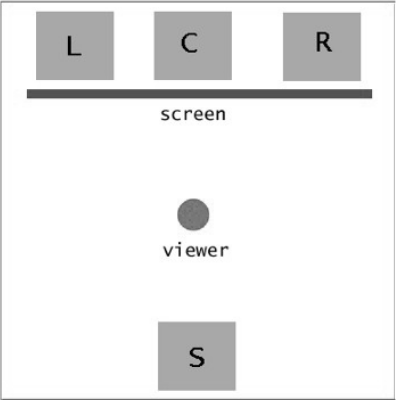
\includegraphics[width=0.3\textwidth]{Images/Dolby Stereo channel configuration.png}
    \caption{Configuration des canaux du Dolby Stereo \parencite[p.~42]{kerins_narration_2006}}
    \label{fig:Dolby Stereo channel configuration}
\end{figure}


\begin{figure}[ht]
    \centering
    \hspace*{-1cm}
    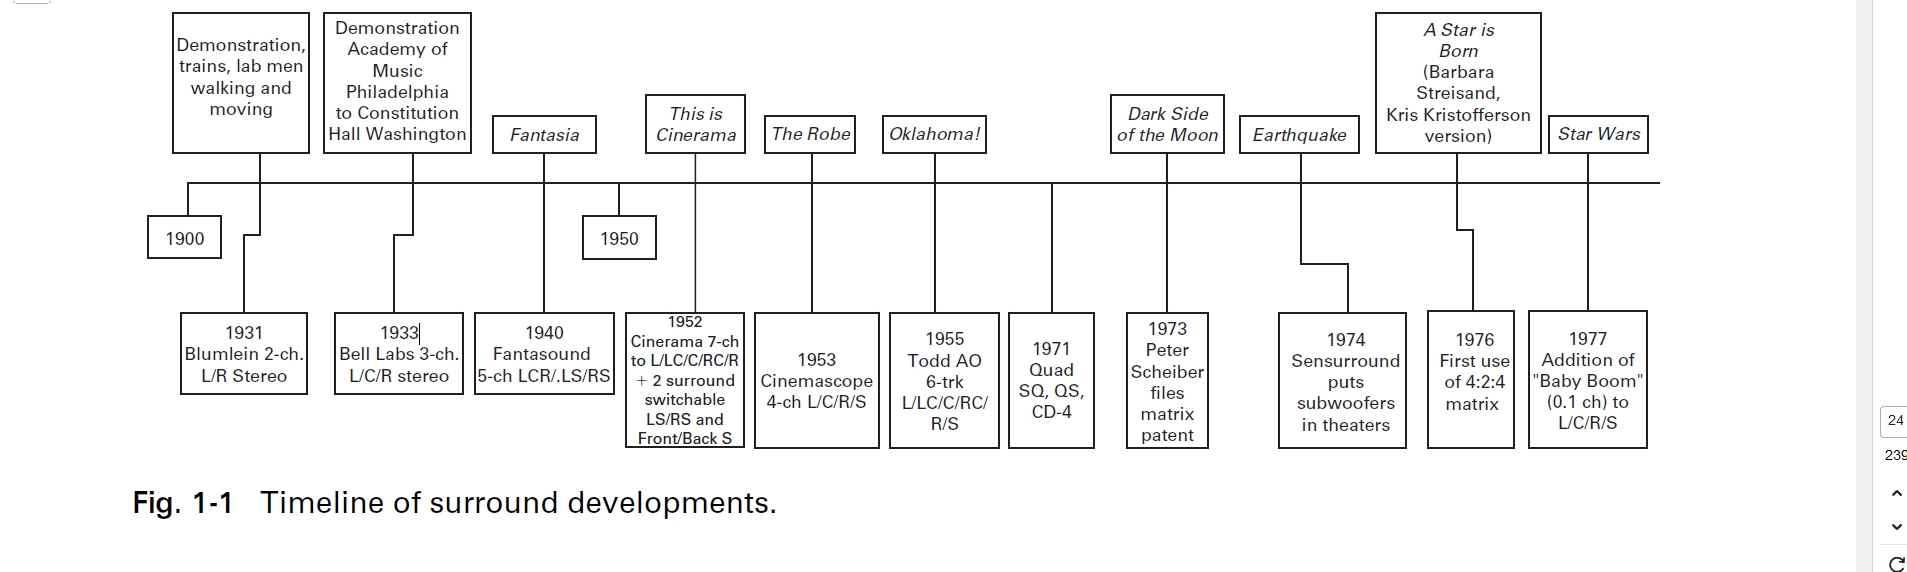
\includegraphics[
        width=1.1\textwidth,
        trim=3cm 2cm 2.5cm 0,
        clip
    ]{Images/Timeline of surround developments 1.png}

    \vspace{0.5em}
    \hspace*{-1cm}
    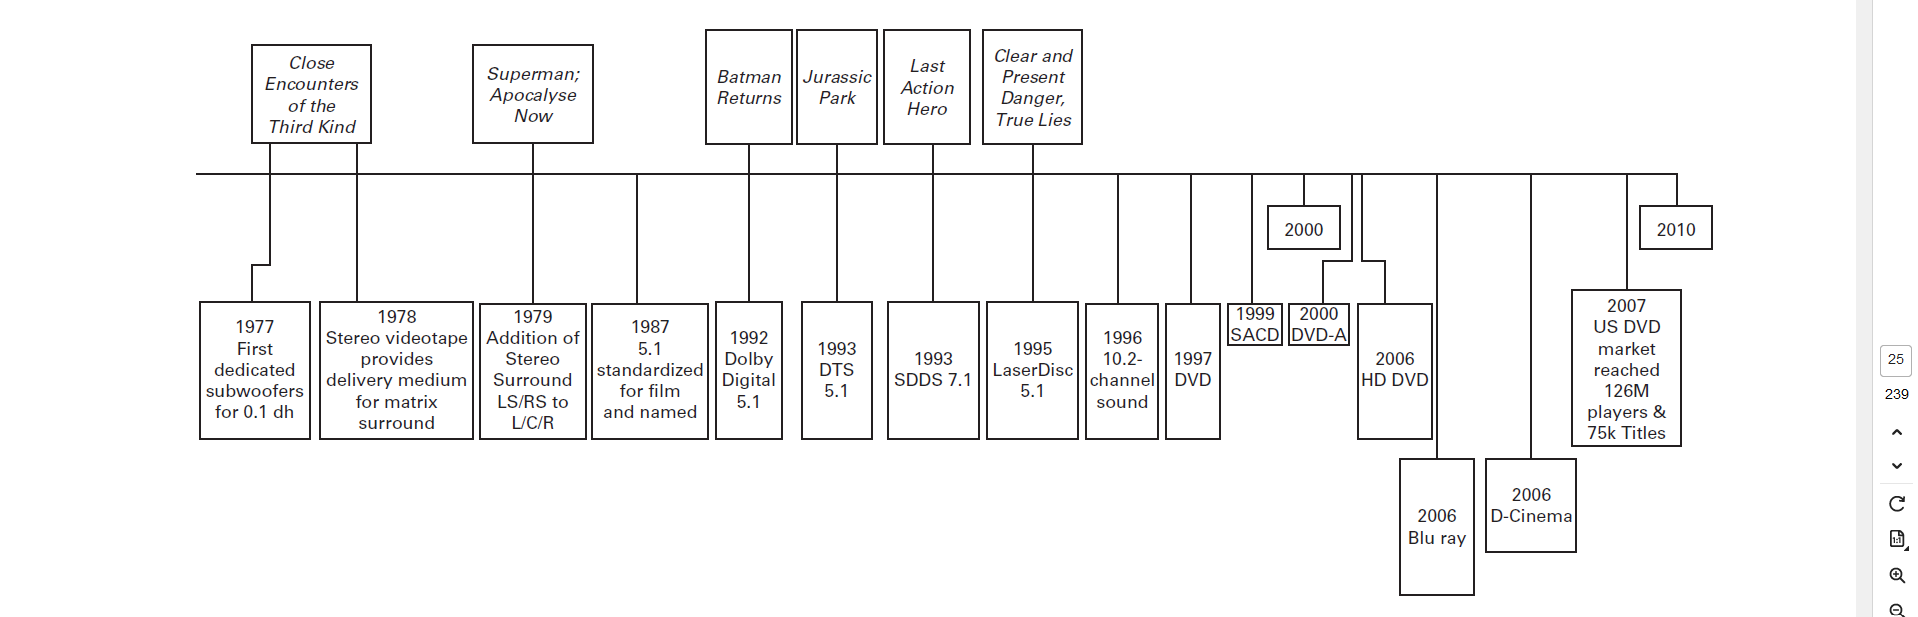
\includegraphics[
        width=1.1\textwidth,
        trim=3.5cm 0.3cm 2cm 0,
        clip
    ]{Images/Timeline of surround developments 2.png}

    \caption{Frise chronologique des développements du son multicanal \parencite[pp.~20--21]{holman_surround_2008}}
    \label{fig:Timeline of surround developments}
\end{figure}

\textcite{adjiman_usages_2018} date l'apparition de l'ambiance sonore dans la bande-son des films (bien que de manière ténue) aux années 1950 et note leur prise d'importance croissante 20 ans plus tard à l'arrivée du son multicanal dans la plupart des films sortants en salle. Le son multicanal au cinéma n'a d'ailleurs ensuite jamais cessé d'évoluer avec par exemple l'émergence des systèmes de diffusion \textit{5.1}, \textit{7.1} ou encore \textit{Dolby Atmos}\footnote{Cette technologie permet d'étendre les systèmes multicanaux traditionnels en ajoutant une dimension verticale et en permettant le positionnement d'objets sonores dans un espace tridimensionnel}. Le besoin de remplir ce nouvel espace sonore toujours plus important et l'envie d'exploiter les nouvelles possibilités qu'il offre expliquent donc en partie cette évolution des pratiques.

L'accroissement considérable de la dynamique\footnote{Écart entre le son le plus faible et le son le plus fort} des bandes-son rendu possible par différents progrès technologiques a lui aussi contribué à la prise d'importance de l'ambiance. La réduction du bruit de fond en est un bon exemple. Des technologies comme \textit{Dolby A}\footnote{Premier système de réduction de bruit professionnel créé par Ray M. Dolby à la fin des années 1960 \parencite{de_nanteuil_dictionnaire_2008}}, permettant la réduction du souffle de la bande magnétique ou optique \parencite{denizart_lemergence_2017}, ou encore la digitalisation du signal sonore \parencite{adjiman_usages_2018} ont permis d'améliorer le rapport signal/bruit. L'amélioration des systèmes de diffusion en salle ont également contribué à cette évolution \parencite{adjiman_usages_2018}. Ainsi, on a pendant le montage son la possibilité de mettre en scène des couches sonores d'ambiance plus faibles en terme de niveau sonore, et donc parfois plus subtiles, discrètes.

L'apparition d'un canal de basses fréquences dédié (\textit{LFE}) dans les systèmes multicanaux a elle permis d'élargir la bande fréquence des systèmes de diffusion vers le bas \parencite{denizart_lemergence_2017} et a donc amené les monteurs et monteuses son à utiliser, créer et mettre en avant des ambiances pouvant comprendre des sons comprenant des basses fréquences.

Pour finir, l'évolution de la perception et des exigences des spectateurs et spectatrices est aussi à prendre en compte.  Par exemple, \enquote{le silence total serait un vide numérique totalement incompréhensible et dérangeant pour le spectateur contemporain} \parencite{adjiman_usages_2018}, c'est pourquoi on monte maintenant des \textit{fonds d'air}\footnote{\enquote{Ambiances très légères [aussi] appelées des silences plateau [...]. Elles s'apparentent à un presque silence, à un souffle. Mais aussi faible soit-il, ce dernier donne déjà des indications sur le lieu, il signe l'espace. De plus il conserve toutes les caractéristiques de l'ambiance, il est une trame, un substrat sur lequel vont pouvoir se poser des événements sonores saillants et des voix} {p.~5} \parencite{adjiman_semiotique_2015}}. \enquote{Au-delà de la question du silence, "le spectateur lui-même a été habitué à entendre davantage de sons qu'auparavant". Il n'accepte plus d'être soumis à un arrière-plan toujours totalement sobre et stylisé, composé de quelques sons symboliques sur lesquels émergent bruits, paroles et musiques. Un certain réalisme sonore domine aujourd'hui ; même dans les cas les plus épurés, le fond est tissé d'un tapis subtil qui habite l'espace} \parencite{adjiman_usages_2018}.

\subsubsection{Le vent comme ambiance naturelle : définitions et caractéristiques}

\paragraph{D’un point de vue descriptif}
 
\parencite{gaver_what_1993} (p.24), 
\parencite{krause_wild_2002} p.38 vent pas entendu directement, P.53 terme musical  p.50, 61, 94, 139-141
\parencite{chattopadhyay_auditory_2021} p.91 le vent peut amener, porter des sons 
\parencite{chattopadhyay_auditory_2021} ex de narrations : p.94

\paragraph{D’un point de vue scientifique}

\paragraph{Du point de vue des professionnels du son}

\leavevmode

Le vent peut tout d'abord être défini comme une texture sonore proche d'un bruit blanc mais présentant des micro-évènements (bourrasques, variations d'intensité...) affectant plusieurs bandes fréquentielles \parencite{mcdermott_sound_2009}. Il peut également être qualifié comme spectralement large (donc comme un bruit) et sur lequel se superposent des composantes sinusoïdes stochastiques, c'est-à-dire instables, aléatoires dans le temps, ne suivant pas un schéma déterministe répétable, mais une distribution probabiliste stable \parencite{schwarz_state_2011}.

Pour le décrire, on peut aussi évoquer la notion de texture sonore reprise par Schwarz : de multipleséléments sonores élémentaires, survenant de manière périodique, aléatoire ou mixte, dont les caractéristiques globales (timbre et amplitude) restent en moyenne stables sur de longues durées \parencite{saint-arnaud_classification_1995}.

Schwarz distingue deux types de synthèse de textures sonores la synthèse de texture expressive, pour la composition musicale, des performances, ou les arts sonores, et la resynthèse de texture naturelle, c'est-à-dire synthétiser les sons de l'environnement naturel pour le cinéma ou les jeux vidéo, le tout en recherchant un certain degré de réalisme. Dans le cas du vent, c'est cette seconde catégorie qui va nous intéresser. 

Il ajoute aussi que la perception de telles textures sonores repose moins sur la reconnaissance de sons ponctuels que sur la texture globale. L'utilisation de la synthèse granulaire semble alors une solution intéressante pour recréer cette texture tout en offrant la possibilité de moduler plusieurs caractéristiques de notre ambiance de vent.

\subsection{Les outils existants}

\subsubsection{Les synthétiseurs d’ambiances naturelles existants}

\subsubsection{Les différents types de synthèses}

\paragraph{Synthèse additive et soustractive}

\leavevmode

La synthèse additive repose sur un principe constructiviste : le son est élaboré en superposant un grand nombre d'oscillateurs sinusoïdaux, chacun représentant une fréquence, une phase et une amplitude distinctes. Conformément au théorème de Fourier, toute forme d'onde complexe peut théoriquement être reconstituée par la somme de sinusoïdes élémentaires \parencite{farnell_designing_2010}.
Chaque composante peut disposer de sa propre enveloppe de volume et d'un point d'entrée et de sortie indépendants, ce qui confère à cette méthode une précision analytique élevée, particulièrement adaptée à la modélisation de corps rigides percutés dont le contenu spectral évolue de manière
contrainte dans le temps \parencite{farnell_designing_2010}. 

Une variante courante consiste à ne pas assembler des sinusoïdes pures, mais à superposer des formes d'onde plus complexes --- dents de scie, triangles, impulsions ou bruits --- issues d'oscillateurs analogiques. Cette approche, caractéristique des premiers synthétiseurs analogiques tels que le Moog ou les machines Roland et Korg, permet d'obtenir une grande variété de timbres musicaux avec un nombre limité de sources \parencite{farnell_designing_2010}.
 
La synthèse par table d'ondes (\textit{wavetable}) constitue une alternative intermédiaire : en substituant les sinusoïdes élémentaires par un large répertoire de formes d'onde enregistrées, elle réduit la complexité du paramétrage tout en conservant la logique d'assemblage additive. Popularisée dans les années 1990 par des instruments tels que le Roland JV-1080 ou le Korg Wavestation, cette méthode reste cependant tributaire des enregistrements disponibles et nécessite une mémoire de stockage importante, ce qui la distingue des approches véritablement procédurales \parencite{farnell_designing_2010}.
 
La synthèse soustractive procède d'une logique inverse : plutôt que de construire le son par accumulation, elle part d'une source spectralement riche (typiquement du bruit blanc) et en soustrait les composantes indésirables par l'application de filtres \parencite{farnell_designing_2010}. Farnell propose la métaphore de la sculpture : de même que le sculpteur retire la matière superflue du bloc de marbre pour révéler la forme qui s'y trouve, le synthétiste soustrait des fréquences pour dégager la couleur
sonore recherchée. Cette analogie soulève toutefois une limite fondamentale : si le matériau
de départ ne contient pas les composantes spectrales nécessaires --- autrement dit, si le bloc de marbre comporte des lacunes --- le résultat escompté ne peut être obtenu, quelle que soit la précision du geste \parencite{farnell_designing_2010}.
 
Dans la pratique, la synthèse soustractive s'appuie sur des filtres résonants capables non seulement d'atténuer certaines bandes de fréquences, mais également de les amplifier, créant ainsi des colorations spectrales caractéristiques. Il convient de rappeler que, dans le domaine des signaux audio, toute amplification relative d'une fréquence équivaut à une atténuation de toutes les autres \parencite{farnell_designing_2010} : le spectre sonore constitue un système de rapports, non de valeurs absolues. La maîtrise des filtres --- passe-bas, passe-haut, passe-bande, coupe-bande --- ainsi que de leurs paramètres de coupure et de résonance, est donc centrale dans cette approche. Les synthétiseurs Surge et Z3TA+, notamment, illustrent la richesse des possibilités offertes par des architectures de filtrage élaborées, combinées à des tables d'ondes et à des oscillateurs multiples \parencite{cann_how_2007}.
 
En définitive, synthèse additive et soustractive représentent deux paradigmes complémentaires de la construction sonore : l'une procède par assemblage méthodique de composantes élémentaires, l'autre par révélation progressive d'une forme à partir d'une matière brute. Leur opposition n'est pas seulement technique, mais aussi épistémologique, en ce qu'elle reflète deux conceptions distinctes de la créativité sonore --- l'une analytique et cumulative, l'autre sculpturale et réductive. 

Dans la conception sonore contemporaine, ces approches sont souvent combinées au sein d'un même instrument ou d'un même patch. Leur distinction devient davantage heuristique qu'opératoire \parencite{farnell_designing_2010, cann_how_2007}.

\paragraph{Synthèse granulaire}

 It is common understanding that sonic phenomena of textural nature – such as the sound(s) of the rain, cracking of rocks and icebanks, thunders, electrical intermittent noises, the sound(s) of the wind, various kinds of “sonorous powders”, burning materials, rocky sea shores, certain kinds of insects, etc. – are best modelled by microstructural time-based design strategies, rather than spectral modelling strategies (see examples in [13][14][15], and musical considerations in [16][17], where granular synthesis methods were employed) \parencite{di_scipio_synthesis_1999}


\paragraph{Synthèse par modélisation physique}

\subsubsection{Audio procédural}

\subsubsection{Protocoles de contrôle}

\paragraph{Le MIDI}
\paragraph{L'OSC}
\paragraph{Divers autres}

\newpage

\section{Cahier des charges}

\subsection{Entretiens avec des professionnels}

\subsection{Établissement du cahier des charges}

\newpage

\section{Conception du synthétiseur}

\subsection{Techniques utilisées}

\subsubsection{Synthèse granulaire}

\paragraph{Vent "pur"}

\paragraph{Éléments additionnels}

\subsubsection{Synthèse additive et soustractive}

\subsubsection{Reverbs et réponses impulsionnelles}

\subsubsection{Utilisation de sons enregistrés}

\newpage

\section*{Conclusion}
\addcontentsline{toc}{section}{Conclusion}

\newpage

\printbibliography

\newpage

\appendix

\section{Transcriptions d'entretiens}
\subsection{Entretien avec Théo Serror}
\setlength{\parindent}{0pt}
\textbf{N : Nohan Bresson}
\textbf{T :Théo Seror}  
\\

\textbf{N :} Alors déjà, est-ce que tu peux te présenter succinctement : ton métier, les projets sur lesquels tu travailles en général, ton parcours étudiant et professionnel, et le nombre d'années d'expérience que tu as dans le métier ? 

\textbf{T :} Je m'appelle Théo Seror, je suis monteur son, j'ai 30 ans, je suis sorti de l'école Louis Lumière en 2018, donc ça va faire 8 ans, et je suis monteur son quasi exclusivement pour le cinéma, pour le long métrage de fiction. 

\textbf{N :} Ou de documentaire au cinéma. OK. Alors, est-ce que tu utilises des outils de synthèse et/ou de sampling — des plugins, des synthés — pour concevoir des sons sur tes projets ? Et si oui, est-ce que tu peux citer un ou plusieurs exemples de situations, de projets dans lesquels tu as utilisé ça ? 

\textbf{T :} Ouais, alors je m'en sers — je dirais — tout le temps, dans presque tous les contextes, que ce soit pour des sons dits réalistes ou des sons qui seraient dits fabriqués. C'est pas une dichotomie qui m'est très utile en pratique. Je l'utilise dans tous les contextes, que ce soit pour un film naturaliste ou un film de science-fiction. Pour parler des outils plus précisément, celui que j'utilise le plus, c'est le sampler intégré à SoundMiner qui s'appelle Radium. Ensuite, des outils communs de sampling — encore une fois — ou de synthèse granulaire, qui sont deux choses assez proches il y a Undertone et Sound Particles, ainsi que Space Grain de DGRM Tools. Et après, une quantité de synthétiseurs, mais là on peut aller les voir. 

\textbf{N :} OK. Est-ce que tu peux citer des exemples ? En fait, tu t'en sers sur quasiment tous les films sur lesquels tu travailles, du coup on peut juste regarder ta filmographie. OK. Tu avais commencé à répondre un peu à ça tout à l'heure, mais du coup, tu t'en sers pour un peu tout type de son des effets, des ambiances naturelles, des nappes ? 

\textbf{T :} Ouais, exactement. Et vraiment, il n'y a ni de morphologie ni de fonction narrative qui soit spécifique à l'utilisation de tel ou tel outil. C'est juste un chemin pour aller du son qui est dans ma sonothèque jusqu'à l'idée que j'ai dans la tête. 

\textbf{N :} Ouais, OK. Et du coup, en parlant de ces sons dans la sonothèque, est-ce que des fois tu te sens limité par l'utilisation de banques de sons lorsque tu dois monter des ambiances ? Et si oui, à quel niveau tu te sens limité ? 

\textbf{T :} C'est difficile... On est toujours limité, parce qu'il y a toujours une distance entre les sons qu'on a sous la main et l'infinie diversité des émotions et des sensations. Après, comment dire, évidemment j'ai pas tous les sons du monde dans ma sonothèque. Donc régulièrement, il manque une nature, ou une couleur, ou une certaine densité, ou une certaine configuration particulière, une certaine distance particulière qui correspondrait spécifiquement à la scène sur laquelle je suis en train de travailler. Généralement, c'est juste des lieux où je n'ai pas encore enregistré. 

\textbf{N :} Du coup, pour continuer à ce niveau-là, quelle est ton approche du montage des ambiances, notamment concernant les différentes couches que tu poses et leur rôle ? C'est un peu large comme question, mais est-ce que, quand tu crées ces ambiances en synthèse, tu crées ça pour des besoins spécifiques ? Ou est-ce que ça comble toutes les caractéristiques que tu imagines pour la scène ? Ou est-ce que tu fais ça vraiment en plusieurs couches, plusieurs étapes ? 

\textbf{T :} Je vais essayer de trouver une façon structurée de répondre à la question. Il y a plusieurs choses. Le premier obstacle, c'est que je suis bien embêté de faire la différence entre les ambiances et les effets dans la réalité du montage. C'est peut-être une particularité personnelle, parce que d'autres collègues font peut-être la distinction de façon plus claire. Moi, des fois je sais pas bien ce qui est un effet, ce qui est une ambiance, à quel moment on passe de l'un à l'autre. Du coup, je me pose pas trop la question. On peut éventuellement faire la différence entre les sons qui sont à l'image et ceux qui ne le sont pas, mais même ça, c'est pas toujours utile — et surtout, il y a pas de différence dans la façon de les fabriquer, a priori. Pareil sur la morphologie des sons les ambiances, ce seraient des sons continus ? C'est pas évident. 
Mais ensuite, pour ce qui est de comment on les fabrique et quelle stratégie on adopte, ce qui est certain, c'est que pour des raisons qui tiennent aux nécessités de mise en scène d'une part et aux nécessités techniques du mixage d'autre part, on a besoin de séparer les éléments sonores. On a besoin que les objets sonores soient distincts et discriminés, que ce soit en termes de densité, fréquentiellement, ou en termes de plan sonore. On prend tout le temps l'exemple des vents ou des foules. Pour les vents, si je monte des vents, je vais essayer de monter séparément des sons qui vont prendre en charge le bas du spectre, d'autres qui vont prendre en charge l'énergie — la sensation d'énergie —, donc plutôt le médium, et puis d'autres sons qui vont prendre en charge le détail ou la violence et qui seront plutôt dans l'aigu ou l'extrême aigu. Il en va de même pour les foules je monterais des sons qui prendraient en charge la masse, la sensation de quantité de gens et de densité — donc sans doute des sons d'un plan un peu plus lointain, peu intelligibles — et puis j'irais petit à petit vers des sons plus intelligibles, sûrement enregistrés avec moins de gens, jusqu'à des trucs plus ponctuels où on discerne des mots, qui permettent de donner du relief à l'ambiance. Et là, c'est plus un découpage séquentiel, c'est plutôt un découpage spatial de la profondeur. 

\textbf{N :} Bah oui, c'est vraiment intéressant, ça répond à pas mal de points que j'avais, donc cool. Et du coup, pour continuer — par rapport à ce que tu disais sur créer ces ambiances — est-ce que quand tu les crées, tu les crées en temps réel en lisant la vidéo ? Et si oui ou non, pourquoi ? 

\textbf{T :} Ça dépend. En gros, la vidéo c'est ce qui donne l'image, et donc le montage d'image, c'est ce qui donne le rythme et la narration. Donc c'est indispensable, et il y a plein de fois où c'est pertinent de travailler avec. Mais il y a aussi plein de fois où je crée des ambiances, où je fabrique des sons avec un sampler, un synthé, comme j'enregistrerais des sons avec un micro et un enregistreur. C'est-à-dire que je vais en faire plein, qu'ensuite je vais dérushes, et qu'ensuite je vais monter. Parce qu'en en faire plein de façon un peu libre, ça va me donner des idées. Il va peut-être y avoir des accidents et ça va peut-être m'emmener quelque part. Ça me permet aussi d'explorer la variété des sons que je peux fabriquer avec le dispositif que j'ai sous les doigts. Et l'autre raison, c'est que faire correspondre les sons au montage des images — aux valeurs de plan, à l'énergie de la scène, à la narration, au point d'écoute, etc. — c'est quelque chose de très précis que je n'ai généralement pas l'habileté de faire en temps réel. 

\textbf{N :} OK. Donc la question suivante, c'était sur les outils de synthèse que tu utilises, mais tu as déjà pas mal répondu à ça. Ensuite, est-ce que tu utilises des périphériques de contrôle, des claviers, des contrôleurs ? 

\textbf{T :} Ouais, tout le temps. Moi j'ai un clavier MIDI avec un certain nombre de potentiomètres rotatifs, une molette de modulation et une molette de pitch. Et avec ça, on fait les choses. Des fois, si j'ai un iPad dans la salle, ça peut m'arriver de faire des choses avec un écran tactile. Parfois, si j'ai envie de m'amuser, je peux brancher une pédale d'expression, mais... De toute façon, il n'y a pas tant de paramètres que ça que mon cerveau est capable de discriminer à la fois sans que ça commence à me demander un effort qui me déconnecte de la narration. Parce que l'instrument change à chaque fois. C'est pas comme si j'avais une pratique établie : quand je joue de la flûte par exemple, j'ai suffisamment appris l'instrument pour oublier ce que font mes doigts et penser à la musique ou à ce que raconte l'histoire. C'est moins le cas quand mon instrument change tout le temps, parce que des fois c'est un vent, la fois d'après c'est des foules, la fois d'après c'est du tonnerre, la fois d'après c'est des battements d'ailes, et que les paramètres que je modifie — une fois le pitch, la fois d'après un filtre, la fois d'après la vitesse d'un Doppler, etc. 

\textbf{N :} Ouais, d'accord. OK. Donc tu as déjà un peu répondu aussi concernant la raison — pourquoi utiliser des outils de synthèse plutôt que des banques de sons, et dans quelle situation ? 

\textbf{T :} Ah non, je pense pas y avoir répondu. À ton avis, pourquoi j'y aurais déjà répondu ? 

\textbf{N :} Parce que tu avais déjà dit que des fois c'était juste qu'il n'y avait pas les éléments que tu imaginais ou que tu recherchais dans tes banques de sons, et que du coup... 

\textbf{T :} Ah non, c'est pas pour ça. Non, c'est vraiment pas pour ça. Ce que tu vas pouvoir faire avec les outils de synthèse ou d'échantillonnage — bon, ça change les sons — mais ils conservent une communauté d'esprit avec les sons que t'avais déjà. Il n'y a rien que tu fais avec un sampler que tu pourrais pas faire en micro-montage, avec des plugins et de l'automation. Donc c'est pas la nature des sons qui est vraiment en jeu. S'il y a des sons qui me manquent dans ma sonothèque, la solution c'est plutôt d'aller les enregistrer. 
Donc en fait, la différence fondamentale qu'introduisent particulièrement les outils d'échantillonnage, en relation avec un contrôleur MIDI par exemple, c'est la performance. C'est de retrouver un geste et une performance dans la fabrication du son qui ne soit pas justement celle du cliquer-glisser, d'empiler des sons dans une timeline et devoir faire play pour les écouter. Non, au contraire. Et c'est précisément à ça que ça me sert — précisément pour ça que je m'en sers tout le temps et quels que soient les sons le sampler me permet de jouer les sons en temps réel. Par exemple, si je joue un son avec une note et que je veux en entendre plus, je peux jouer plusieurs notes à la fois. Ça me permet d'augmenter la densité et de sentir tout de suite ce que ça produit comme différence, d'essayer plus aigu, plus grave, plus vite, moins vite, etc. C'est vraiment le rapport au geste et à la performance qui pour moi fait la différence principale. Parce que, encore une fois, il n'y a rien que je fais avec un sampler qui me serait absolument inaccessible par du montage et de l'automation. 

\textbf{N :} OK, donc ce serait plus le côté pratique et le côté concrétisation de ce que tu imagines et de ce que tu veux créer ? 

\textbf{T :} Ouais, exactement. Et c'est vraiment le rapport à la performance — c'est aussi le fait d'avoir un geste, d'avoir un engagement physique. Tu bouges tes doigts, tu joues le truc. Ça permet d'avoir une frontière en moins entre l'idée et sa réalisation. C'est comme la différence entre mixer au fader et mixer au crayon dans la timeline. Je dis pas qu'il y en a un qui est meilleur que l'autre, mais ça fait des trucs différents. Il y en a un qui permet de connecter une sensation physique — la position de ton doigt sur la console — à une sensation — le volume qui rentre dans tes oreilles. Et là, c'est pareil. Et du coup, quand tu le fais face à l'image, d'un seul coup tu peux jouer le son en même temps que tu regardes l'image. C'est pas toujours ce qu'il y a de plus pratique, mais parfois je vais m'entraîner en regardant l'image et après enregistrer sans la regarder. Ça te permet d'avoir une connexion entre le son et ta sensation physique. 

\textbf{N :} OK, trop intéressant, ça répond à pas mal de trucs aussi. Alors la question suivante : dans quelle situation tu utilises des outils de ce genre ? 

\textbf{T :} Ambiances, effets, bruitages, sons naturels, sons de synthèse — ouais, il y a pas de distinction particulière. 

\textbf{N :} Et est-ce que tu utilises ça à un certain moment de la postproduction, à un certain moment de ta prise en charge du montage ? Est-ce qu'il y a un certain timing ou est-ce que c'est plus ou moins libre ? 

\textbf{T :} Évidemment, ça dépend des films, ça dépend des conditions de montage, du temps que j'ai, etc. A priori, j'ai plutôt tendance à écouter beaucoup de sons et à dérushes beaucoup de sons avant de commencer à monter — pour avoir en gros tous les sons possibles en tête avant de commencer à les monter, et que les sons que je choisis soient bien celui qui me plaît le plus parmi tous ceux que j'ai à disposition, et pas le premier que j'ai trouvé. Donc ça demande un peu de temps, mais quand je suis dans ces conditions-là, la fabrication des sons intervient après la première phase de dérushage — c'est-à-dire après avoir écouté tous les sons, sélectionné tous ceux qui me semblaient pertinents pour le film ou la scène en question. Et là, une fois que j'ai récupéré tous ces blocs, je vais commencer à jouer avec. C'est une façon de faire, et ce serait une étape qui interviendrait juste avant d'effectivement monter les sons. 
Mais ensuite, ça arrive quand même que pendant le montage, pendant l'assemblage — quand je commence à mettre des sons sur la timeline, en face des images, etc. — il peut m'arriver que d'un seul coup j'ai une idée qui me vient, et dans ce cas-là je la réalise tout de suite. C'est pour ça que je compare la fabrication des sons à l'enregistrement. Ça vient du même endroit créatif, ça vient s'accrocher aux mêmes envies, à la même énergie et aux mêmes nécessités. Donc, de la même façon que je vais plutôt enregistrer les sons pour une scène avant de monter la scène, j'ai toujours un micro dans ma salle, et si j'ai besoin d'enregistrer un son tout de suite, je vais le faire au moment où j'en ai besoin. Les deux existent à la fois, et il y a même des allers-retours il peut m'arriver de monter une scène, de me rendre compte qu'il me manque des sons, et de m'organiser pour aller les enregistrer — parfois des jours ou des semaines plus tard — pour les ajouter à la scène en temps voulu. C'est pareil avec la fabrication des sons. 

\textbf{N :} Et est-ce qu'il y a des types de scènes, des types d'environnements ou des types de sons en particulier qui reviennent régulièrement, pour lesquels tu utilises des synthétiseurs ou des plugins ? 

\textbf{T :} Ouais, il y a quelques trucs un peu récurrents. Pour la synthèse granulaire — Undertone, etc. — les foules, c'est vraiment un cas récurrent. Ça me permet, par exemple, à partir d'un son qui ne serait pas suffisamment long, pas suffisamment dense, et éventuellement un peu trop intelligible, de faire des sons plus longs, plus denses et moins intelligibles. Le cas typique, c'est genre : j'ai un son de conversation qui dure une minute, qui est bien mais qui est un tout petit peu trop intelligible. Du coup, il ne peut faire que le premier plan sonore. Et à côté de ça, j'ai des sons à moi qui n'appartiennent pas au film, qui ont donc une autre couleur, qui sont un peu plus lointains, et qui peuvent me servir pour faire le plan très large. Eh ben, Undertone va me permettre de prendre ce son seul, de le mettre dedans, et à partir de ça, de faire une espèce de 2e ou 3e plan sonore qui fera le lien entre ce son du film et mes sons qui ont une couleur un peu trop différente. 

Après, Space Grain, par exemple, c'est un truc dont je me sers très souvent pour donner à partir de sons un peu trop statiques — un son qui aurait plus de relief dans le temps et dans l'espace. Et ça peut être de la foule comme ça peut très bien être des sons complètement abstraits — des cendres qui volent, par exemple. 


\textbf{N :} Et du coup, de manière un peu générale, dans ton utilisation de ce genre d'outils, est-ce que tu pourrais donner les principaux avantages et inconvénients ? 

\textbf{T :} C'est un peu comme dire : c'est quoi l'avantage et l'inconvénient d'un marteau ? C'est pas pour moi une grille d'analyse qui m'est très utile pour évaluer les outils. Genre, effectivement, avec un marteau c'est super pour planter des clous, c'est beaucoup plus chiant pour enfoncer des vis. Mais est-ce que c'est vraiment un inconvénient du marteau ? Peut-être dire « limitation » plutôt qu'inconvénient. Non, il s'agit vraiment de remarquer ce que ça peut faire et ce que ça ne peut pas faire. Comme une chaise : c'est bien pour s'asseoir, on peut éventuellement grimper dessus pour être plus grand, mais c'est dangereux et pas stable. Et pour construire des murs, ça ne marche pas. 
Donc, qu'est-ce que ces outils permettent de faire ? Pour les samplers — genre Radium — ou les synthés réintroduire du geste et de la performance dans la fabrication des sons. C'est vraiment pour moi le truc crucial. Il y a un mouvement, il y a une intensité. Je peux jouer le son plus fort, moins fort, plus vite, moins vite, plus dense, moins dense — et le faire non pas en ayant besoin de le conscientiser à l'avance, puis de le réaliser, puis de l'écouter, mais vraiment en le ressentant et en l'entendant tout de suite. C'est vraiment le truc crucial du sampler avec un clavier ou un autre contrôleur — comme un bruitage ou comme quand on enregistre des sons —, tout en conservant la possibilité de changer les sons qu'on met dans le sampler et d'avoir un fort degré de granularité et de contrôle. 
L'autre chose, ça me permet d'ajouter ou de soustraire des qualités à des sons que j'aurais déjà. Dans le cas d'Undertone, les rendre plus longs, plus larges, moins précis, plus denses. 
Ce que ça ne fait pas, c'est le montage à ta place. Ça n'arrive jamais que je joue quelque chose du début à la fin de la séquence et que je le laisse tel quel. Ça n'arrive pas, parce que le montage n'est pas aléatoire. Le montage du film, la narration du film — on ne fait pas du jeu vidéo. Il y a un déterminisme dans le déroulé de l'expérience du spectateur : il voit toujours le film dans le même sens et dans le même ordre. Et par conséquent, il y a un déterminisme de la bande son. Sinon, c'est que je n'ai pas fait mon travail de savoir ce que je raconte, à quel instant du film, ce que ressent le personnage, ce que je veux que ressente le spectateur. Les monteurs et monteuses d'images, les réalisateurs et réalisatrices ne font pas leurs coupes au hasard. 

\textbf{N :} Oui, tu suis déjà quelque chose. 

\textbf{T :} Ouais, exactement. 

\textbf{N :} OK, trop bien. Et après, tu as cité beaucoup d'outils que tu utilises. Est-ce qu'il y a des contrôles ou des fonctions — des types de synthèse, des types de paramètres — que tu trouves particulièrement utiles dans ceux que tu utilises ? Et à l'inverse, est-ce qu'il y en a qui manquent ou auxquels tu as déjà pensé ? 

\textbf{T :} Ouais, je sais pas trop. Ces outils sont très différents les uns des autres — il y a pas grand-chose en commun dans le fonctionnement entre Undertone et Radium par exemple. Mais si on parle des outils d'échantillonnage, un truc que je trouve très utile, c'est la possibilité — quand tu charges plusieurs couches de son — d'avoir du suivi d'enveloppe entre les différentes couches. C'est un des meilleurs moyens de les faire fusionner, de donner la sensation que c'est un seul son et non plusieurs superposés, pour pouvoir les contrôler en même temps. Et surtout que l'enveloppe d'un des sons puisse contrôler le volume d'un autre — un vrai suiveur d'enveloppe. Ça, c'est un outil que je trouve vraiment utile. 
C'est pas comme ça que j'évalue les outils je m'attends pas à ce qu'un seul outil fasse tout. Cela dit, ça n'empêche pas de penser à des outils dont on rêverait. Il y a quand même des situations, notamment pour les trucs génératifs. T'as entendu parler de Vandaval ? 

\textbf{N :} Non, je crois pas. 

\textbf{T :} Ah, pourtant je pensais t'en avoir parlé, parce qu'au début ton sujet portait sur les vents génératifs. Bref, c'est un moteur de synthèse de vents gratuit qu'un développeur a fait — je pense dans Max — et qui existe en Audio Unit et en VST. Et ça, par exemple, c'est vraiment chouette : ça te permet de faire des vents en les construisant à partir de paramètres narratifs et perceptifs. Tu conçois le vent dans ta tête, et tu as des sliders qui correspondent non pas à des paramètres physiques, mais à des questions du genre : est-ce qu'il est sifflant, pas sifflant, fort, pas fort, varié, pas varié, etc. Ça te permet d'avoir un truc qui est proche de la façon que tu as de ressentir les choses. 
Et donc, en gros, un outil dont on rêve — on est plusieurs à rêver de ça depuis très longtemps — c'est quelque chose de similaire pour les foules tu pourrais fabriquer le son de foule avec des sliders pour la densité, l'émotion, l'énergie, le volume, l'espace dans lequel ça se passe, la distance, le niveau d'intelligibilité, etc. C'est là que je trouve qu'on a des manques réels. 

\textbf{N :} Si tu me l'avais conseillé, je viens de le retrouver. 

\textbf{T :} Ah oui, je m'en rappelle maintenant. Je t'invite vraiment à l'essayer en plus — c'est un VST gratuit, c'est assez simple, ça fait très bien ce qu'on s'imagine que ça peut faire. Il y a aussi Wind Machine, dans le même genre. 

\textbf{N :} Ouais, ça je m'en rappelle. 

\textbf{T :} Bah, Wind Machine, je m'en sers pas. Vandaval, je m'en suis un peu servi — et en même temps, c'est pas de ça dont je me sers le plus souvent quand j'ai besoin de faire des vents. 

\textbf{N :} Ouais, tu gardes l'option d'avoir plusieurs outils différents — c'est plus intéressant que d'avoir un outil spécialisé unique ? 

\textbf{T :} Non, au contraire : plusieurs outils qui sont très spécialisés. Par exemple, Vandaval — ça m'arrive de m'en servir, mais ça ne fait jamais l'intégralité du vent. Mais au contraire, je préfère avoir plusieurs outils spécialisés qu'un outil qui me permet de tout faire — de la même façon que j'aurais pas envie d'avoir un seul instrument pour l'orchestre. On ne demande pas à un violon de faire de la batterie. Dans ma boîte à outils, j'ai plusieurs outils et j'ai pas juste un Leatherman. 

\textbf{N :} En plus, j'imagine que plus tu les utilises, plus tu connais leurs capacités et tu sais comment les utiliser. 

\textbf{T :} Ouais, exactement. Et ça a à voir avec un concept qui s'appelle l'affordance — c'est-à-dire l'utilisation que suggère spontanément un outil ou un objet. Par exemple, une chaise : spontanément, tu vas la mettre sur ses quatre pieds et tu vas te dire que tu peux t'asseoir dessus. Tu la mettras pas les pieds en l'air pour essayer de t'en servir comme d'un escabeau. Ça, c'est l'affordance de la chaise. Pareil, l'affordance d'un piano : spontanément tu vas pas ouvrir le capot d'un piano à queue pour aller gratter les cordes, tu vas plutôt appuyer sur les touches. Pareil pour la guitare : l'affordance de la guitare, c'est plutôt de pincer les cordes que de taper sur le manche. 
C'est un concept qu'utilisent beaucoup les gens dans le monde du design, d'interface utilisateur ou d'expérience utilisateur — l'UI/UX —, particulièrement dans le monde du numérique, pour voir comment faire pour que l'utilisateur sache que telle partie du programme, il peut cliquer sur tel menu pour qu'il se déroule, tirer sur la fenêtre pour l'élargir, etc. Donc l'intuitivité et l'ergonomie ont une importance dans les outils. 
Ce que je veux dire, c'est qu'il y a une utilisation qui est inhérente, une façon spontanée d'utiliser un outil — c'est une volonté de la personne qui l'a fabriqué. Et c'est pas mal en soi qu'un outil préconise une utilisation spécifique et que ce soit ça que tu ailles explorer. Plutôt qu'un outil qui se croirait neutre, où tous les boutons feraient la même taille, complètement austère, et qui ne te dirait pas comment s'en servir. Alors ça peut te laisser libre d'une certaine façon, mais prisonnier d'une autre. Un tournevis sans manche, par exemple. 
Et donc, quand on fabrique des outils créatifs, il y a une intention créative dans l'outil — et ça, il convient de l'assumer. Ce n'est pas une limite en soi. Ou ça n'en est pas plus que de dire qu'un violon, ce n'est pas bon pour faire de la batterie.

\textbf{N :} Oui, c'est inhérent à ce qu'on fait dans tous les cas. 

\textbf{T :} Oui, exactement. 

\textbf{N :} OK. C'est tout pour mes questions. Merci beaucoup, ça m'a vraiment éclairé — d'autant plus par rapport aux autres entretiens que je vais faire, donc ça m'a bien fait avancer. 

\textbf{T :} Trop bien. Bonne continuation, et hésite vraiment pas. Bonne journée. 

\textbf{N :} Toi aussi. Merci, salut. 


\subsection{Entretien avec Guillaume Bouchateau}
\setlength{\parindent}{0pt}
\textbf{N : Nohan Bresson 
} 
\textbf{G : Guillaume Bouchateau}  
\\

\textbf{N :} Déjà, merci de répondre à ce petit entretien.

\textbf{G :} Je t'en prie.

\textbf{N :} Je voulais commencer par savoir si tu pouvais te présenter succinctement : ton métier, les projets sur lesquels tu travailles en général, ton parcours étudiant et professionnel, et les années d'expérience que tu as dans le métier.

\textbf{G :} Alors, dans l'ordre. Mon métier : chef monteur son, sound designer — j'aime bien « chef monteur son », ça me va très bien. Sur quels films je travaille ? En général, sur des gros films internationaux. Je fais autant de films français que de films étrangers, même s'ils sont souvent coproduits par des Français, mais ils sont souvent à destination internationale. Que de la fiction, oui, et que du long-métrage. Je fais très peu de télé — j'en ai fait un peu à un moment parce que j'avais des réalisateurs qui en faisaient, mais j'en fais plus. Parcours étudiant : j'ai fait la Fémis, il y a longtemps. Je suis rentré en 95, sorti en 97 ou 98, quelque chose comme ça. Et j'ai travaillé tout de suite. En fait, j'ai même fait mes heures pendant la Fémis, parce que je travaillais le soir. En dernière année, on a moins de cours, donc j'en ai profité pour valider mes heures.

\textbf{N :} Est-ce que tu utilises des outils de synthèse et/ou de sampling — que ce soit des plugins ou des synthétiseurs, du hardware physique — pour concevoir des sons sur tes projets ? Et si oui, est-ce que tu pourrais citer un ou plusieurs exemples récents ?

\textbf{G :} Alors, ça dépend à quoi tu penses, parce que la synthèse en tant que telle, ça marche pas forcément seul — ça se combine. Les sons que j'utilise... je vais prendre un exemple simple sur un film que j'ai fait : je vais citer Lucy, par exemple, ou Valérian. Quand t'as beaucoup de sons à fabriquer — des vaisseaux spatiaux, des drones, des robots, des trucs comme ça — c'est très souvent des mélanges de plein de choses. C'est-à-dire que tu vas prendre un son concret que t'as enregistré, tu vas faire un peu de bruitage bidouillé, plus des sons de synthèse. Le truc avec la synthèse, c'est que je pars très souvent d'un son original. C'est très rare que je parte d'oscillateurs.

\textbf{N :} Tu te bases sur des sons de ta banque que t'as enregistrés, essentiellement ?

\textbf{G :} Oui. Alors après, je peux utiliser des sons et les passer dans plein de bébêtes, plein de bidules — ça je peux le faire. Mais en général, j'utilise assez rarement des sons de pure synthèse. Ça peut arriver, mais c'est très rare, sauf quand j'ai des interfaces numériques à faire, ou des pistolets laser ou des choses comme ça. C'est pas assez complexe, ni assez vivant. Après, moi j'ai très tôt utilisé le sampler pour fabriquer des sons. Je me souviens qu'à l'époque, début 2000, il y avait pas beaucoup de plugins. Il y a un truc que j'arrivais jamais à faire et qu'on mettait des heures à faire, c'était des mouvements ou des Doppler. Pour faire ça, il fallait d'abord faire un fade, puis changer le pitch, puis faire des reverbs — c'était compliqué. Et moi, j'avais acheté un émulateur uniquement pour la fonction Doppler. C'était le premier sampler qui avait un vrai truc comme ça. Et puis après il avait des filtres et des choses comme ça, mais je passais des sons concrets dedans. J'étais plus dans une logique de sampling que dans une logique de synthèse. Et c'est toujours le cas.

\textbf{N :} Quand tu utilises des outils de synthèse, est-ce que c'est plutôt pour certains types de sons — des effets, des ambiances naturelles, des nappes ?

\textbf{G :} Des effets, des ambiances naturelles — il n'y a rien qui vaut une ambiance naturelle. Je vais pas mettre un bruit rose avec un filtre piloté par LFO pour faire la mer, jamais. Sauf quand je veux faire un effet particulier et qu'on est dans un film de science-fiction et que tu veux faire un hommage à Alien. Mais sinon, non, ça marche pas pour moi. Dans un film naturaliste, je vais jamais utiliser ça. Je préfère passer beaucoup de temps à trouver le bon son. Une belle couleur acoustique — des Atmos, des choses comme ça — il n'y a rien de tel.

\textbf{N :} Est-ce que ça t'arrive de te sentir limité par l'utilisation des banques de sons lorsque tu dois monter des ambiances ?

\textbf{G :} Les banques de sons, c'est un outil parmi d'autres, mais en général on a enregistré nos sons nous-mêmes et c'est vachement mieux. On a toujours des manques sur des choses très particulières, peut-être, mais quand je me sens en manque de quelque chose, je vais en réenregistrer. C'est beaucoup plus simple que de me faire chier à essayer de faire un machin où je vais mettre une semaine pour faire un truc qui va ressembler vaguement à quelque chose de naturaliste.

\textbf{N :} Et quelle est ton approche du montage des ambiances, notamment concernant les différentes couches et leurs rôles ?

\textbf{G :} Alors, ça dépend du film. Je parle pour un film plutôt naturaliste, un film normal. J'ai toujours à peu près 3 couches d'ambiance : 2 que je monte dans les ambiances et une que je monte dans les effets. Je vais t'expliquer pourquoi. La toute première, c'est vraiment un fond d'air, un fond qui caractérise une pièce, qui permet de raccorder les paroles — avec un bon centre, un truc très neutre, mais qui change de couleur en fonction des intérieurs, extérieurs, etc. C'est mes assistants qui m'en fabriquent. J'en ai fabriqué à la pelle : pour des grandes pièces, des petites pièces, des extérieurs, des mers, des forêts, des villes. C'est très neutre, mais ça permet toujours de raccorder la sous-couche — le fond de sauce, quoi. On n'est pas loin d'un bruit rose ou d'un bruit blanc, un peu modulé, un peu trafiqué. Ça me donne tout de suite une couleur : dedans, dehors, jour, nuit — bêtement. Et puis après, je mets une couche d'ambiance vraiment plus spécifique, mais assez floue, assez large, qui a déjà des caractéristiques. Et après, je peux monter par-dessus les détails dans les effets. Par exemple pour de la pluie : je vais monter un fond très bas, puis des détails de gouttes qui donnent la force de la pluie, et tous les détails je vais les monter dans les effets, goutte par goutte. Il y a un fond de base de pluie très large et très loin qui donne le tour, avec un petit fond orageux dans les fonds d'air de base. En deuxième couche, je mets la pluie drue avec la couleur bitume — une pluie par terre. Et puis dans les effets, je vais monter un peu de flaque et un peu de métal s'il y a un balcon à droite, par exemple. Je vais panner les gouttes sur le balcon à droite. Et là, j'ai mon ambiance. De toute façon, il faut tout décomposer. Moi, je décompose tout, je propose un équilibre — les niveaux, les pannes, les reverbs — et après, ça se voit au mix. Le mixeur reçoit des stems en 7.1 Atmos ou en 5.1, et il en fait ce qu'il en veut : soit les filtrer, soit jouer sur les épaisseurs de son. Et s'il veut rentrer dans l'intérieur de mes équilibres, il peut aussi le faire, parce que les pistes ne sont pas brassées — elles sont accessibles.

\textbf{N :} Est-ce que tu crées en lisant la vidéo pour le faire en direct ?

\textbf{G :} Ça dépend. En général, j'aime bien me préparer des choses. Le problème des outils de synthèse, c'est qu'automatiser, c'est chiant — c'est trop lourd. Donc j'aime bien me préparer des trucs je sais que je vais avoir besoin de certains passages, je les prépare, j'affine, je randomise l'audio, je rebricole, et je reviens dessus. Le seul truc où je faisais ça en direct, c'était un outil qui s'appelait Grip — en fait un logiciel qui était pas un logiciel de synthèse, plutôt de sampling à l'image, où il y avait que des sons de pneus qu'on pouvait trafiquer, panner. Et là, je calais ça à l'image en fonction de la position, en pannant. Sinon, je vais me servir d'Igniter, des Krotos — je vais pas m'amuser à automatiser ça devant chaque bidule. Je me fais plutôt une grosse sonothèque avec des passages, des textures constantes, différentes, et après je les réécole en montage — c'est plus simple pour moi.

\textbf{N :} Est-ce que tu peux citer les outils de synthèse ou de sampling que tu utilises le plus souvent ?

\textbf{G :} Les Krotos et les UVI. UVI, c'est assez pratique. Des fois des trucs comme Unlokt ou comme Footsteps, parce que c'est carrément des sons concrets que tu peux traficoter et ça tu peux le faire à l'image. C'est pas vrai pour les flingues aussi, ou pour les coups — des fois sur des armures avec les Sound FX d'UVI, je me suis amusé à les faire tout à l'image, avec un clavier MIDI, t'envoies des infos MIDI et tu cales tes trucs.

\textbf{N :} Est-ce que tu utilises des claviers ou des contrôleurs ?

\textbf{G :} J'en ai toujours un dans ma salle, depuis 20 ans. Un clavier MIDI un peu général — la vieille M-Audio de base. Il y a un vieux Novation avec plein de boutons dont je me sers plus, mais avant je m'en suis servi parce que c'était bien piloté et bien mappé. Je peux m'amuser à jouer avec un filtre et une enveloppe si j'ai envie. Mais encore une fois, on ne fait pas de musique — ça n'a rien à voir avec ce que je peux faire quand je fais de la musique. Et ça donne des couleurs très typées en fait. Même quand j'utilise les UVI, les risers, les astéroïdes et les trucs comme ça, je m'en sers pour faire des mouvements — je me fais une couche avec Asteroid, j'en fais 3 ou 4 différentes, je vais me faire 2 ou 3 autres couches avec autre chose, et après je mélange.

\textbf{N :} J'imagine que tu les gardes pour les projets suivants, ces effets que t'as créés ?

\textbf{G :} Alors oui, je les garde, mais je les réutilise jamais. Je refais parce que c'est jamais pareil en fait — t'as d'autres idées, t'as d'autres outils. J'ai fait des trucs avec de vieux outils, des fois après tu les changes, t'en refais d'autres. C'est plus facile de garder des bases, tu vois. Je me suis fabriqué des bases que j'utilise toujours — j'avais sampleté des trucs d'Aphex Twin que j'avais tripotés dans tous les sens, ça je les garde parce qu'il y a une couleur qui est dingue. J'ai fait quelques impacts sourds, je peux m'en resservir. Et puis les versions de Pro Tools changent toujours, elles ne sont plus compatibles avec les mêmes plugs — ils vont passer sur Rosetta, donc il faut refaire la dette du plug. Donc tes presets sont bons, mais toutes les valeurs ne sont pas forcément importables.

\textbf{N :} Dans quel type de scène, dans quelles situations particulières utilises-tu ces synthés ?

\textbf{G :} En général, c'est pour des sons plutôt ponctuels et percussifs. Des fois pour faire des espèces de sons de néons, des trucs un peu électro. Des rumbles aussi. Et sinon des sons un peu ponctuels, ou quand tu as des trucs vraiment très particuliers. Après, j'utilise beaucoup d'autres outils — moi je trouve que la granulaire marche très bien en général. Donc je me sers beaucoup de... comment ça s'appelle... ce plug qui est génial, chez Audio Ease — voilà : Undertone. Ça j'utilise beaucoup. Sinon c'est pour des effets purement de sound design des mouvements, des impacts ou des choses comme ça, pour gonfler certains sons. Je sais que j'avais fait sur Dracula, quand le personnage se tape sur les armures avec la main au début du film — je manquais de trucs. Donc j'avais utilisé beaucoup les armes Krotos et les Sound FX d'UVI, et en les samplant avec différentes hauteurs, en les jouant au clavier, ça faisait un effet de masse. Pour épaissir, mais pas tout seul — tout seul, ça sonne « pouet pouet ».

\textbf{N :} Est-ce que tu crées ces sons à un certain moment de la post-production — en amont, ou sur le moment ?

\textbf{G :} Là, il y a pas de règles — ça dépend des films. Là, je fabrique des sons avant parce que j'ai un temps de prépa j'ai 4 semaines de prépa avant de démarrer le film. Il y a aussi tout un moment où tu passes ton temps à regarder tes logiciels — ce que je fais en ce moment. Tu regardes des logiciels, tu fais un son, tu essaies de comprendre comment ça marche, tu te dis « Tiens, il y a un truc marrant. » Faut que ça mature, quoi. Moi, je plonge pas bille en tête en me disant « Je vais faire un son de machin. » Je peux essayer de faire un son, et puis après ça me plaît pas forcément. Je mets des espèces de templates que j'appelle des tests — des tests de son. J'en fais 5 par type de son, ou 6, ou 20, peu importe. Et puis après je reviens dessus, je me dis « Est-ce que c'est intéressant ? » Et là, je peux décliner dans différentes directions. Il y a pas de règle ça dépend des films, ça dépend de tes envies, ça dépend des besoins du film, ça dépend de plein de choses.

\textbf{N :} Est-ce que dans les outils que tu utilises, il y a des fonctions ou des contrôles que tu trouves particulièrement utiles ou intéressants ?

\textbf{G :} Bah en fait, ce que j'utilise beaucoup... quand je pense à Unlokt, ou à Walker, Whoosh, des trucs comme ça chez UVI — ou Stream FX — c'est vraiment fait pour nous. C'est plus des outils de sampler avec un filtre, un peu d'effets — des trucs simples, avec des macros sur les caractéristiques des sons. D'abord c'est des sons concrets, donc la forme d'onde c'est du sampling amélioré. En gros, c'est comme quand tu utilises Kontakt, tu vois — dont je peux me servir aussi. Mais en gros, j'ai besoin d'une courbe d'enveloppe, d'un filtre résonant. Les effets embarqués en général, je les trouve pas bien — je les refais moi, parce que je vais les séparer éventuellement. Ce que j'aime bien faire, c'est empiler les couches en changeant les pitches, en changeant la hauteur — ça suffit pour grossir le truc.

\textbf{N :} Tu préfères quand même rentrer dans la maîtrise des enveloppes et des filtres plutôt qu'utiliser les contrôles globaux proposés parfois par les plugins ?

\textbf{G :} Ça dépend. Encore une fois, je vais être chiant, mais il y a pas beaucoup de règles. Ça dépend de ce que je veux faire. Mais encore une fois, tous ces trucs-là, que ce soit sur Kontakt ou chez UVI, t'arrives assez vite à trouver tes trucs. Maintenant on peut même utiliser Radium directement sur Soundminer — t'as ta sonothèque dedans, et il y a déjà des macros sur Radium pour certains usages. Antoine a dû t'en parler. Pour les mers, on a déjà fait des trucs avec des macros sur Radium et des choses comme ça — c'est vachement bien. Je trouve ça pratique. Je trouve ça un peu usine à gaz, moi, mais c'est parce que je suis vieux, je crois.

\textbf{N :} Est-ce qu'il y a des remarques que tu t'es faites sur des fonctions qui manquent, que t'aurais envie de voir sur tel plugin ou tel synthé ?

\textbf{G :} Oui, j'ai toujours des demandes. Je trouve que les utilisations du pitch ne sont jamais très satisfaisantes dans un sampler ou un standalone en général, parce que comme ça dépend de la vitesse de lecture, c'est toujours compliqué. Moi, je voudrais qu'il y ait des variations de pitch qu'on puisse caler en fonction de l'image. Par exemple : tu fais une voiture, t'as un moteur de voiture, tu veux l'accélérer un peu — tu fais une automation, tu le ralentis. Et pour que ça se joue automatiquement, que tu puisses dire « la fin de mon moteur est là, l'arrivée de la voiture est là », et que le moteur monte et descende automatiquement — ce genre de trucs. Ça rejoint un peu ce que j'avais fait avec Grip, avec les trucs de sampling et de pitch, surtout de variation de hauteur. Ce que je voudrais, c'est un truc qui soit un mélange entre Move It — le plugin panoramique de HAL — et la gestion des pitches. Antoine, il s'arrache les cheveux avec ça, c'est trop compliqué à cause de la vitesse de défilement de l'image. Parce que quand tu fais une variation de pitch dans un synthé, tu la fais dans le moteur du synthé et tu l'envoies dans ton DAW — après c'est calculé, ça bouge plus. Ce que je veux, c'est pouvoir ajuster la vitesse de lecture d'un son en temps réel dans l'image.

\textbf{N :} Et c'est compliqué à implémenter ?

\textbf{G :} C'est très compliqué. Ou alors il faut avoir le plugin en insert sur la piste — mais même là, le problème c'est que c'est lié à une vitesse de défilement. Si t'as une vitesse de défilement qui varie en fonction de l'image, tu peux faire varier ta hauteur mais pas ta longueur. En parlant d'un vari-speed, oui — je comprends, mais c'est vrai que c'est une bonne remarque.

\textbf{N :} Mon mémoire porte sur l'utilisation des outils de synthèse pour la création d'ambiances naturelles spécifiquement. Je fais des entretiens avec des monteurs son et des sound designers.

\textbf{G :} Alors je te dis ça, je m'en suis quand même un peu servi pour fabriquer des mers. Avec du granulaire — beaucoup. On s'en est servi pour deux choses. C'était d'abord pour faire des ambiances de ville qu'on n'avait pas. C'est-à-dire, j'avais un New York 1930 à faire. Et on s'est amusé — et ça marchait assez bien — à récupérer de vieux enregistrements d'époque et on les a passés dans Undertone, pour les élargir, pour les avoir plus longues, plus nombreuses. Il y avait des sons de Manhattan en 1930 — qui avaient un son un peu dégueulasse, mais qu'on a pu nettoyer au maximum avec iZotope. Même si on n'avait pas des fréquences très élevées, c'était quand même exploitable. On en a mis plusieurs pour faire un peu du multicanal. Et franchement, ce qui était très intéressant, c'est que quand tu regardais le film, on avait des ambiances disons normales et jolies avec des vieilles voitures. Mais on avait des fonds un peu jolies et par-dessus on avait mis des passages de vieilles voitures qu'on avait enregistrées très proprement, pour donner la couleur, le côté rétro. Et ça nous donnait un truc absolument unique. Quand tu mélangeais les trois, tu te disais « Mais c'est dingue, on y est ! » Parce qu'il se passe un truc très bizarre : ton cerveau, quand il voit un film des années 30, il entend le son des années 30 avec lequel il a grandi — le son des films qu'on voyait des années 30. Si tu mets un son un peu dégueulasse, ça le choque pas. C'est hyper intéressant. Et j'ai fait ça aussi pour des sons de mer, parce que j'ai fait un film qui se passait sur un bateau essentiellement. C'était compliqué parce qu'on avait enregistré beaucoup de mer au bord, même des rochers, des trucs très bien enregistrés. L'ingénieur du son direct a fait plein de beaux sons sur le bateau — on entendait le bateau — mais on voulait de la mer large, des fois sans avoir le bateau. Et pour ça, j'ai utilisé ce qu'il avait fait au bord de l'eau avec des grands mouvements de micro pour que les vagues soient plus grosses. Et ça, tu le passes dans Undertone, dans un granulaire, tu peux éventuellement un peu filtrer.

\textbf{N :} Oui, j'avais déjà entendu des ingénieurs du son parler de ce problème-là — de ne pas avoir la mer au large sur le bateau.

\textbf{G :} Eh ben, ça, on l'a complètement fabriqué pour le film sur Florence Arthaud. Ça marchait super bien. On avait fait des essais avec différentes longueurs de grains — des couches de longs, des couches de courts, justement. Ça dépendait si on voulait que ça bouge. Le truc, c'est que quand tu fais des grains trop longs, tu sens les crossfades, tu sens les coupes. Et comme c'est du bruit rose, c'est assez compliqué. On avait mis beaucoup de couches. Mais ça marchait bien. C'est intéressant parce que ça résolvait un vrai problème. L'ingénieur du son direct avait fait tout ce qu'il pouvait — il avait fait des trucs super. Il disait : « Le seul truc que je pourrais jamais avoir, c'est de la mer large, sans bruit. » Il a fait des essais, il est même parti sur un Optimist — mais il pouvait pas aller loin, et puis ça fait tout de suite du bruit.

\textbf{N :} C'est intéressant aussi parce que ça implique de penser à cette étape du montage dès la prise de son.

\textbf{G :} Très intéressant, ça je m'en suis servi. Mais c'est pas ce que j'appelle des outils de synthèse pour moi. C'est du sampling — tu rentres du sampling et tu fais de la granulaire dessus. On s'amusait à prendre des stéréos, des monos, à les rentrer et à repanner les choses. Et ça c'est pas mal parce que ça donne vraiment un truc où tu peux faire des mouvements avant-arrière, c'est super. Tu crées directement ton image, tu joues tes mouvements de panne. D'ailleurs, c'est une fonction qui n'existe pas, mais moi j'aimerais bien qu'on puisse associer des fonctions de détection de hauteur spectrale avec des fonctions panoramiques. Pour avoir, par exemple, les graves devant — ou inversement — pour faire un passage grave-aigu sur une vague. Quand les aigus sont au centre, tu fais des passages comme ça — t'as des mouvements dans tous les sens, ça bouge. Et on ressent toujours un effet de Doppler dans les oreilles. Ça pourrait être la même chose pour le vent, le feu, les feuilles — tout ce qui est bruit rose.

\textbf{N :} Bah ouais, intéressant. Bon, c'est tout ce que j'avais comme questions — merci, c'était très cool d'avoir ton retour là-dessus.


\textbf{G :} Bon courage pour la suite. Ciao !

\subsection{Entretien avec Aymeric Devoldère}
\setlength{\parindent}{0pt}
\textbf{N : Nohan Bresson 
} 
\textbf{A : Aymeric Devoldère}  
\\

\textbf{N :} Déjà, merci de bien vouloir m'accorder ce temps alors que c'est un peu le rush, j'imagine. Est-ce que tu peux te présenter succinctement — ton métier, le rôle que tu as en général sur les films, le type de projet sur lequel tu travailles régulièrement, ton parcours étudiant et professionnel ?

\textbf{A :} Je m'appelle Aymeric Devoldère, je suis chef monteur son depuis longtemps, depuis bientôt 30 ans — enfin, un peu moins de 30 ans quand même. Je fais surtout du long-métrage, mais je peux faire aussi de la série, enfin un peu tout, et sur tout type de film — que ce soit de la fiction, du documentaire, des films d'auteur, des films à effets. Je suis pas cantonné à un style. C'est même ça qui est agréable, de pouvoir passer d'un univers à l'autre avec des besoins et des demandes différentes à chaque fois. Et mon parcours — j'ai fait Louis Lumière et j'ai fait la Fémis. Je suis rentré à Louis Lumière en 91, sorti en 93, puis rentré à la Fémis dans la foulée. Donc sorti en 97. Après, aujourd'hui je fais que du montage son, mais pendant longtemps j'ai cumulé les deux casquettes. Je faisais à la fois de la prise sur les tournages — j'ai beaucoup travaillé en binôme avec Lucien Balibar, j'étais à la perche. Et en général quand on travaillait ensemble, c'est plutôt moi qui prenais en charge le montage son, mais Lucien était monteur aussi. On a fait ça pendant un moment, et puis bon, par intérêt — parce que le montage son a toujours été ce qui m'a le plus intéressé — à un moment j'ai arrêté de faire de la prise de son. 

\textbf{N :} Est-ce que tu utilises des outils de synthèse et/ou de sampling — des plugins ou des synthés — pour concevoir des sons sur les projets sur lesquels t'es ? Est-ce que tu peux citer un ou deux exemples d'utilisation récemment ? 

\textbf{A :} J'utilise pas mal tous les outils qu'a créés Antoine pour UVI — que ce soit Drone, enfin tout ça, tous ces outils-là je peux les utiliser. Ça m'a incité, à un moment où je le faisais plus beaucoup, à me racheter un clavier, à pouvoir jouer les sons. L'autre outil que j'ai un peu utilisé, c'est Extreme FX. Ça a été un peu comme avec Antoine — on s'est retrouvés à travailler un peu ensemble, on est devenus associés, et ça a été un peu le redéclencheur de ça. Mais ça se cantonne à des utilisations assez particulières, faut vraiment en avoir besoin pour vraiment designer des choses. Je les utilise plutôt en sous-couche — sur Auto Drone, j'aime bien l'utiliser pour ajouter quelque chose, comme une sorte de passerelle entre le montage son et quelque chose de plus musical. Là sur ce film-là — 223 fois — je l'ai utilisé un peu en layer supplémentaire du score. Ça se joue pas à des niveaux devant, mais ça rajoute, ça permet de mêler un peu plus le montage son et les musiques quand c'est possible. 

\textbf{N :} C'était justement ma question suivante — est-ce que tu l'utilises plus pour des effets, des ambiances naturelles ou des nappes ? 

\textbf{A :} Oui, c'est plus des nappes. Quand il faut créer un effet de bulle, ou qu'on a envie que tout d'un coup le point de vue se subjectivise un peu — j'aime bien l'utiliser comme ça. Et de pouvoir le jouer, c'est intéressant, parce que même en manipulant quelques paramètres en direct, on peut tout de suite avoir quelque chose d'assez vivant, de pas statique. Mais c'est plus dû à la façon de jouer le son qu'à l'outil en tant que tel. On retrouve quelque chose de plus direct, de plus intuitif quand on fait ça sur un clavier — ce qui est assez agréable — alors qu'au montage son c'est extrêmement laborieux : c'est une couche, faut en rajouter une autre, on ajuste la première, puis la deuxième, puis la troisième, et ça se construit comme ça. 

\textbf{N :} C'était aussi un des points qui m'intéressait pour mon mémoire — la variation des techniques de travail dans le montage son. Des fois l'intérêt des synthés, juste en termes d'amusement, de côté un peu différent, de changer de méthode de travail, ça peut être intéressant. 

\textbf{A :} Oui, vraiment. Ça faisait longtemps que je le faisais pas — pas par volonté, juste parce que j'avais pas forcément les outils. Et donc là je me suis racheté un petit clavier et je m'en sers vraiment régulièrement. Même sur Extreme FX — par exemple pour poser des bases. Sur Emilia Pérez, j'avais une grosse séquence de fusillade à faire avec Extreme FX. Ça a pas fait le son complet, mais ça m'a permis de trouver — j'avais au moins 3 grandes couleurs à trouver. J'ai posé des bases comme ça, puis après je les ai évidemment complétées, et il en est resté quelque chose. Et je suis allé assez vite — ça m'aurait pris plus de temps de le faire en cherchant et en collant les sons. Le son était pas fait, mais en termes d'intention, il y avait quelque chose. On retrouve un peu une logique de bruiteur, qui va faire quelque chose d'un peu plus live que ce qu'on fait au montage son — ce qui est à la fois le plaisir, parce qu'on peut tout contrôler, mais en même temps c'est tellement laborieux par moment qu'on peut vite s'y perdre. Et des fois l'idée, l'intuition qu'on peut avoir sur le moment — elle est pas forcément parfaite, mais elle peut avoir une certaine justesse. 

\textbf{N :} Est-ce que ça t'arrive de te sentir limité par la seule utilisation de ta sonothèque pour des ambiances ? 

\textbf{A :} Non — enfin, on en a jamais assez. Et puis l'idéal, c'est de pouvoir continuer à faire des sons, et encore mieux de les faire pour le projet sur lequel on travaille — c'est quand même toujours sans doute la meilleure solution. En tous les cas sur des films où on a un rapport un peu naturaliste, ça reste toujours une solution très pertinente. Et puis c'est toujours agréable de manipuler des nouveaux sons, surtout quand on a quelques années derrière soi. Même si j'utilise des trucs que j'utilise depuis longtemps, d'avoir toujours de nouvelles matières, c'est super. 

\textbf{N :} Dans les outils que tu utilises précisément — quel type de plugin, de synthèse ou de sampling ? 

\textbf{A :} Alors, le sampling — je l'utilise sans doute fort mal, mais sur des choses un peu particulières, j'utilise le Radium de Soundminer, parce que ça peut aller vite. Je sais pas, une fois j'avais des rats à faire et j'avais pas grand-chose en sonothèque là-dessus. Avec ce que j'avais, j'ai pu faire une espèce de déclinaison assez rapidement avec le sampler et ça marchait assez bien. Après c'est pareil, on peut aller assez vite, accumuler de la matière, après il faut la remonter, la remanipuler. Mais j'en fais pas une utilisation intensive. Après, maintenant dans les sonothèques qu'on fait avec HAL, il y a des patchs dans le Radium qui permettent — sur les dernières collections, Windscape et la collection tout ça — de combiner des choses et de pouvoir les jouer. On l'a utilisé d'ailleurs, puisqu'on avait des séquences de guerre sur ce film-là, avec de grosses explosions sur la mer. On en a fabriqué avec les patchs Radium de la sonothèque qui est sortie au même moment. 

\textbf{N :} Et est-ce qu'il y en a d'autres que tu utilises, un outil de synthèse pure ? 

\textbf{A :} Non, après je sais pas trop ce que tu appelles ça. Des outils de synthèse pure, pas tant que ça. Ou alors le truc de la synthèse, c'est que ça peut pas fonctionner partout — c'est une utilisation très spécifique pour des besoins très spécifiques. Mais par exemple sur les ambiances, puisque c'est ça le sujet — plus ça va, plus je préfère toujours utiliser des sources acoustiques. Partir de quelque chose de réel, quitte à le tordre et à le déformer, à le granuler, à le passer dans un tas de trucs. Les granulaires, ça j'en fais partie aussi — ça je l'utilise quand même beaucoup depuis longtemps. J'utilise beaucoup le Space Grain de GRM, même sur des trucs à priori pas forcément évidents. Ça m'aide notamment sur des histoires de spatialisation, même sur des voix. Par exemple sur le mini APR, je l'ai utilisé beaucoup sur des trucs de marché — il y avait pas tellement de place, et de pouvoir sentir que ça bougeait un peu, je le passais dans le granulaire, pas trop fort pour qu'on entende pas les artefacts. Et par rapport au format Atmos qu'on a maintenant, c'est intéressant. 

\textbf{N :} Tu utilises ce clavier ou d'autres périphériques de contrôle ? 

\textbf{A :} Non, ça suffit, c'est très simple. 

\textbf{N :} Pourquoi utiliser ces outils — c'est quand tu veux augmenter des sons que t'as déjà, rajouter des couches ? 

\textbf{A :} Encore une fois, ça dépend de ce qu'on a à faire. Si je fais un film fantastique, évidemment les besoins vont pas être les mêmes que sur un film d'époque, comme là je fais. Par exemple là, si je me réfère à ce que je suis en train de faire, il y a pas mal de moments où il faut créer des effets un peu subjectifs. Si j'ai l'impression que je vais pas avoir assez de matière avec les sons réalistes de la scène, là je peux assez rapidement me dire : si je peux pas le faire comme ça, faut aller vers quelque chose de plus musical — sans faire de la musique. Mais des fois la frontière peut être très floue. Et c'est bien d'ailleurs — il y a rien de plus agréable que de plus savoir trop qui fait quoi sur un film, quand les choses sont mêlées, quand ça devient un peu organique entre la partition et le montage son. C'est toujours assez agréable. 

\textbf{N :} Est-ce que tu le fais à un moment particulier de la post-production — avant ou pendant ? 

\textbf{A :} Non, pas de règle. Moi, je monte toujours dans l'ordre, donc quand je fais une séquence, je la fais complètement. Après, si t'as un film de SF où il y a vraiment de la matière particulière à fabriquer — comme c'est déjà arrivé — là on se met dans un mode plus de fabrication de son, on est plus vraiment dans un truc de montage pur. C'est ce que les Anglo-Saxons appellent le poste de sound designer — vraiment quelqu'un qui va créer la matière, fabriquer les sons, les inventer, ou trouver un process pour retrouver le truc. Quand nous on emploie le même terme, ça a pas la même signification, mais c'est ça la bonne nomination en fait. En gros ça va arriver sur des films de SF ou des films fantastiques, ou des trucs où il y aura des besoins qui seront, entre guillemets, pas d'ordre réaliste — même si c'est évidemment toujours plus subtil que ça. 

\textbf{N :} Dans les outils que tu utilises, est-ce qu'il y a des contrôles ou des fonctionnalités que tu trouves particulièrement intéressantes ? 

\textbf{A :} Là, je suis pas assez... ces outils-là, je les utilise de façon pas très poussée, parce que j'ai pas vraiment été formé à la synthèse. C'est des outils qui existaient pas du tout quand j'ai commencé à travailler. Je les utilise de façon très basique. Après, quand je trouve quelque chose d'intéressant, je m'en souviens pour les fois d'après. Mais je n'ai pas du tout le rapport de musicien ou de spécialiste avec ces outils-là. Je les utilise sans doute mal d'ailleurs, mais bon. J'essaie d'avoir des idées et de les retranscrire avec les outils que j'ai — j'y arrive plus ou moins. 

\textbf{N :} Il y a des types de contrôles un peu à grande échelle, plus globaux, des fois un peu en mode preset, qui peuvent être intéressants ? 

\textbf{A :} S'il y a pas vraiment ça... ouais, je sais pas trop. 

\textbf{N :} Est-ce que t'as déjà eu un manque, une envie de — « ce serait bien si on pouvait faire ça » — sur un des outils que t'as l'habitude d'utiliser ? 

\textbf{A :} C'est trop général. Après, je me pose jamais vraiment cette question — sans doute parce que j'ai commencé à un moment où tout ça n'existait pas. Enfin, les synthés existaient, mais on pouvait pas les manipuler comme on les manipule maintenant, intégrés à notre outil de travail principal. Non mais c'est peut-être une des spécificités de la post-prod, du son à l'image — il y a plein de façons d'arriver. Il y a le montage son, il y a le bruitage, il y a la musique, le travail sur les voix — je saurais pas répondre à cette question. Après, c'est toujours la même chose, c'est un truc d'expérience. Quand on découvre une machine — comme ça a été le cas quand j'ai pu appréhender tous les outils UVI — j'ai fait des choses que j'avais pas l'habitude de faire avant. Et puis après, on intègre ça dans son workflow interne. Mais il faut pouvoir tester plein de trucs, découvrir des choses — ça prend du temps, et puis faut avoir envie de se plonger dans tout ça. 

\textbf{N :} Quelle est ton approche au niveau du montage des ambiances, notamment concernant les différentes couches et leurs rôles ? 

\textbf{A :} En tous les cas, j'ai toujours pour habitude de commencer par retrouver un fond neutre qui va juste se poser sur la séquence — c'est la première chose que je fais en général. Quelque chose de neutre, juste pour poser l'espace. Et ça, c'est aussi en rapport avec les films qu'on fait en France, qui sont des films énormément basés sur la parole. Donc je garde cette habitude d'ordre. Je pense que je suis pas le seul d'ailleurs. Je pose déjà ça parce que ça va pas être quelque chose de narratif, ça va juste me poser une base de décor, une base d'espace. Et cette tâche, je trouve qu'elle se simplifie largement avec l'Atmos maintenant — avant j'avais l'impression de beaucoup batailler, surtout pour composer avec le 5.1. Maintenant, je trouve que c'est plus facile. Et avec les sonothèques qu'on fabrique avec HAL, ce sont des sons qui peuvent être faits en Atmos natif, donc avec l'Atmos ça marche assez bien. Mais il y a d'autres façons de le faire — en ambisonie, ou on peut fabriquer pas mal de trucs avec Undertone, en bricolant. Tous ces fonds, ce qu'on appelle les fonds d'air — ce qui est peut-être une spécialité française, je suis pas sûr que ce soit autant partagé ailleurs. Donc c'est ce que je commence par faire. Et puis après, c'est le récit qui guide tous les choix. 

\textbf{N :} C'est intéressant, parce que des fois moi quand je monte des ambiances, j'ai l'impression de trop charger — alors que démarrer avec un truc neutre, surtout pour le mix, ça peut donner de la marge. 

\textbf{A :} De toute façon on en a besoin, parce qu'il faut composer avec la parole. C'est pour ça que je disais, cette habitude-là elle est aussi en rapport avec les films qu'on fait — où ça parle. On a besoin d'avoir une base pour asseoir le son direct, et ça permet d'établir ce rapport entre la parole et le son — son direct ou pas d'ailleurs. Moi j'en ai besoin tant que j'ai pas fait ça, j'ai l'impression de pas pouvoir faire la suite. 

\textbf{N :} Et dernière petite question — quand tu crées tes sons avec ces plugins, est-ce que tu le fais en temps réel, en lisant la vidéo, en mode bruitage ? 

\textbf{A :} Un peu, oui. Par rapport à ce que je disais tout à l'heure, si je peux utiliser le clavier, j'essaie de le faire le plus possible à l'image. Après, encore une fois, ça dépend de ce qu'on a à faire. Si on se retrouve sur un film où il y a vraiment de la matière à inventer, là on se met plus dans un mode de recherche qui peut être un peu décorrélé du montage pur à l'image. Mais si j'ai un effet particulier que je peux jouer, ce qui est intéressant c'est justement de pouvoir le faire en temps réel. Après, ça veut pas dire que tu vas pas le retoucher 50 fois, mais d'avoir un premier geste... Ce qui est intéressant, encore une fois, c'est pas tant l'outil en tant que tel que la façon de le manipuler — de pouvoir le jouer. Voilà, le côté souris, couche par couche, son par son — c'est intéressant parce qu'on a l'impression de pouvoir tout maîtriser. Mais il faut jamais oublier qu'on fait du son à l'image, donc plus on a des outils qui nous permettent d'être dans ce rapport-là, plus c'est intéressant. D'ailleurs, c'est pas rare que quand je monte certaines ambiances, j'ai une première idée, je construis comme ça en couches — j'ai fait ça, maintenant je peux rajouter ça, je peux le placer comme ça — en essayant d'être rigoureux pour que ce soit transmissible au mixage, que les mixeurs comprennent ce qu'on a voulu faire. Mais c'est pas rare que le lendemain on réécoute et on se dit « Ah tiens... » parce qu'il y a eu quelque chose de séquentiel dans la pensée, et des fois on additionne des trucs. On peut finir par avoir des effets de masque dans tous les sens parce qu'on a pas assez bien géré l'addition des différentes couches. Et des fois, la somme de ce qu'on a fabriqué correspond pas forcément à ce qu'on voulait. L'enjeu c'est de tout décomposer, mais que quand on regarde la séquence — même si à notre étape de travail la chose est pas mélangée et finalisée — on puisse guider l'écoute et se dire « le son de cette séquence, c'est ça », et qu'on entende pas toutes les couches. Le plus possible. Après évidemment c'est aussi le travail du mixage, mais il faut que ce soit déjà possible. Ce qui compte, finalement, c'est les idées — comment on va pouvoir jouer avec le cadre, les plans, les coupes du montage. 

\subsection{Entretien avec Sylvain Lasseur}
\setlength{\parindent}{0pt}
\textbf{N : Nohan Bresson 
} 
\textbf{A : Sylvain Lasseur}  
\\

\textbf{N :} Alors, je vais commencer par une petite questio\textbf{n :} est-ce que tu pourrais te présenter succinctement, ton rôle en général sur les films, ton métier, et le type de projets sur lesquels tu travailles ?

\textbf{S :} Bon, pour te dire tout de suite, maintenant je suis à la retraite. Ça ne veut pas dire que je ne retravaillerai pas si un film m’intéresse, mais pour l’instant je ne travaille plus depuis six mois.
Avant, j’ai fait comme toi : l’école Louis-Lumière. Ensuite, j’ai fait un peu de perche sur des plateaux de longs métrages. Puis je me suis rendu compte que la post-production m’intéressait davantage que le tournage, même si l’ambiance du plateau est quelque chose de très particulier et d’attirant.
Mais la perche, d’un point de vue travail, c’est très fatigant physiquement, et ce n’est pas très créatif. Donc je me suis orienté vers la post-production. J’ai travaillé en France jusqu’en 2012 à peu près, sur divers films. Le plus simple, c’est de regarder mon profil IMDb, il est à peu près à jour.
En France, j’ai travaillé comme chef monteur son. Ça veut dire que tu fais un peu tout : tu gères l’équipe, tu fais du montage, de la création sonore, du sound design, et tu es l’intermédiaire entre l’équipe, le réalisateur et la production pour tout ce qui concerne le son. Tu portes un peu toutes les casquettes.
Ensuite, je suis parti aux États-Unis parce que je commençais à tourner en rond en France. J’avais envie de nouveaux challenges et d’une nouvelle aventure. Là-bas, j’ai eu la chance de travailler avec un sound supervisor, un rôle différent : lui ne monte pas, ne crée pas de son, il gère l’équipe et fait le lien avec le réalisateur. Moi, j’étais engagé comme monteur son FX editor et sound designer.
La grosse différence, c’est que tu ne t’occupes pas de tout le film, mais seulement d’une partie. Par exemple, sur Deepwater Horizon, je ne faisais que le sound design sous l’eau : les tuyauteries, les explosions, les fluides. Sur Les Huit Salopards, je me suis occupé uniquement du vent.
C’est une autre manière de travailler : tu te concentres sur une tâche précise au lieu d’en gérer des dizaines. Et comme il y a énormément de travail, ça nécessite de grosses équipes.
Le sound design, c’est particulier parce que tu crées des sons qui n’existent pas. Donc tout est ouvert à discussion avec le réalisateur. Ce n’est pas comme un cri d’animal, où tu pars d’une réalité. Là, tu peux expérimenter énormément.
Sur Les Huit Salopards, par exemple, il fallait créer un vent qui respecte le dialogue, très important chez Tarantino. Il fallait qu’il s’adapte, qu’il monte ou descende en fonction de l’intensité des scènes.
Aux États-Unis, j’ai travaillé sur plusieurs films comme Deepwater Horizon, Les Huit Salopards, et Once Upon a Time in Hollywood. C’était une expérience incroyable.
Pour me démarquer là-bas, j’ai mis en avant un outil que j’utilisai\textbf{s :} le Kyma. C’est une machine qui permet de fabriquer ses propres plugins en assemblant des modules. Ça demande de la pratique et des connaissances, mais ça permet de créer des choses uniques.
Par exemple, je pouvais utiliser des suivis d’enveloppe en amplitude et en fréquence, ce qui permet de transformer profondément un son. En sound design, tu es obligé de transformer les sons, sinon ça ne fonctionne pas.
Avec Kyma, tu peux tout faire : nappes, textures, transformations complexes. Tu peux même créer des vocoders, découper un son en bandes de fréquence et en appliquer les caractéristiques à un autre son. Je l’ai utilisé notamment pour des sons d’animaux, en mélangeant différentes sources pour garder un côté organique.
C’est très important que les sons restent organiques, surtout pour des créatures ou des éléments naturels. Même pour un dinosaure, l’oreille doit reconnaître quelque chose de vivant.
Aux États-Unis, peu de gens utilisaient Kyma. Ça a été un vrai facteur différenciant pour moi. J’ai fait une démo, elle a circulé, et ça m’a permis de rencontrer les bonnes personnes et de commencer à travailler sur des gros projets.

\textbf{N :} Et du coup, quel type de sons tu crées avec ces outils ?

\textbf{S :} À peu près tout. Des nappes, des ambiances, des effets… C’est très ouvert. Par exemple, pour les vents, il faut que ça reste organique, sinon ça ne marche pas. C’est même l’une des choses les plus difficiles : transformer un son tout en gardant un rendu naturel.
Kyma m’a permis de faire ça. Je pouvais créer des modules sur mesure, comme des vocoders ou des systèmes où un son en contrôle un autre. C’est une approche que j’aimais beaucoup.

\textbf{N :} Et pour les ambiances, est-ce que tu te sentais limité par ta sonothèque ?

\textbf{S :} Non, mais on n’en a jamais assez. Tu te lasses vite de certains sons. Il faut en avoir beaucoup pour trouver des éléments intéressants.
Moi, je travaillais toujours avec un fond d’ambiance continu, une sorte de tapis sonore, sur lequel je rajoutais des éléments ponctuels. C’est essentiel pour garder de la flexibilité, notamment au mixage. Si un réalisateur n’aime pas un élément, tu peux le retirer instantanément sans tout refaire.
Ça permet aussi de moduler l’ambiance selon l’image, de donner de la vie sans figer les choses.

\textbf{N :} Quand tu utilises tes synthés, est-ce que tu les joues en temps réel ?

\textbf{S :} Oui, ça m’arrive. Par exemple, pour les rafales de vent, je les jouais en direct au clavier en regardant l’image. Ça permet d’interpréter la scène, un peu comme un musicien.
J’utilisais un clavier particulier, le Continuum, où tu peux glisser entre les notes. Ça permet des variations très expressives, notamment pour accompagner les mouvements du vent.
C’est une approche très proche du jeu musical ou du bruitage : tu interprètes en direct, tu recommences si besoin, mais ça apporte une vraie expressivité.

\textbf{N :} Et tu utilisais d’autres outils que Kyma ?

\textbf{S :} Oui, au début, mais à la fin je faisais presque tout avec Kyma. Il permet de faire de la synthèse, de la granulation, du sampling… tout.
Parfois, je préférais le rendu d’un plugin spécifique, mais globalement, j’avais développé tellement de modules que j’avais toujours un outil adapté.
Et puis Kyma a évolué avec le temps. Je travaillais un peu avec les développeurs, je proposais des idées, certaines ont été intégrées plus tard. C’était un outil très vivant, développé par une petite équipe, donc plus lent, mais très flexible.

\textbf{N :} Tu m'avais parlé de ton clavier. Est-ce que tu utilisais d'autres périphériques de contrôle ?

\textbf{S :} Oui, bien sûr. J'ai utilisé une tablette. C'est bien, parce que tu n'appuies pas sur des notes tu as un stylo, tu joues avec, c'est différent. J'ai utilisé aussi des contrôleurs XY, par exemple.
 Le Continuum, tu peux même avoir XYZ : X pour l’horizontal, Y pour le vertical, et Z pour la pression sur la note. Donc tu peux contrôler trois paramètres en même temps avec les doigts. J’ai bossé aussi avec des tablettes, parce que tu peux faire la même chose.
J’ai utilisé aussi des petites consoles pour faire des automations de niveau dans Pro Tools, c’est pratique. Et sinon, pas grand-chose de plus, parce qu’avec ça j’avais déjà tout ce qu’il me fallait.
J’ai testé aussi la Wii, les contrôleurs de mouvement. C’était plus pour expérimenter, avec un ami. On s’est amusés à faire quelques sons, qu’il a utilisés ensuite, mais je ne me souviens plus exactement dans quel contexte.

\textbf{N :} Pour revenir à la synthèse : pourquoi tu utilises des outils de synthèse plutôt que des sons de ta sonothèque ? Et dans quelles situations ?

\textbf{S :} J’utilise la synthèse quand j’ai besoin de modifier un son. Tant que le son me convient tel quel, je prends un son de ma sonothèque. Par exemple, une porte de voiture : si elle est parfaite en tonalité, je l’utilise directement.
Mais si j’aime le son et que je dois l’adapter — par exemple le descendre d’un ton et demi — là je passe par un sampler. Et souvent, ça pose problème : le son devient mou. Donc j’utilise un outil de pitch qui ne modifie pas la durée.
Je n’ai pas de règle stricte, mais je n’utilise pas la synthèse pour créer des ambiances naturelles, sauf cas particuliers — par exemple un vaisseau spatial ou des environnements extrêmes. J’aime que les sons restent organiques, et la synthèse peut vite enlever cet aspect-là, donc il faut l’utiliser avec délicatesse.

\textbf{N :} Est-ce qu’il y a un moment particulier dans la post-production où tu fais ça ?

\textbf{S :} Ça dépend surtout du travail. Aux États-Unis, par exemple, tu es souvent assigné à une tâche précise.
Quand j’étais chef monteur son, si je devais fabriquer un son, je le faisais au moment où c’était nécessaire. Mais souvent, le réalisateur a déjà une idée en tête, surtout pour des sons spécifiques, et il veut les entendre rapidement.
Sinon, tu organises ton travail comme tu veux, sauf en cas de projections intermédiaires. Là, il faut être prêt : synchronisé avec l’image et avec un mix rapide mais présentable, pour que le réalisateur puisse juger et donner son avis.

\textbf{N :} Concernant ton outil de synthèse principal, le Kyma, est-ce qu’il y a des contrôles ou fonctions particulièrement intéressants ?

\textbf{S :} Sur Kyma, c’est moi qui décidais. Je pouvais assigner n’importe quel paramètre à un axe de contrôle. Par exemple, dans la granulation, le nombre de grains plus tu en as, plus le son est dense ; moins tu en as, plus il devient ponctuel.
Je peux contrôler n’importe quel paramètre d’un module, comme dans un plugin. Par exemple, sur une réverbération le temps de réverbération sur X, la taille de la pièce sur Y, etc.
Ensuite, tout dépend de ce que je veux faire. Si j’ajoute un son à une voiture qui passe, je peux faire apparaître les grains au moment où elle est devant, puis les faire disparaître derrière, en jouant aussi sur le pitch. Tout est ouvert.

\textbf{N :} Est-ce qu’il y a des fonctions ou idées que tu aurais aimé avoir ?

\textbf{S :} Non, je n’ai jamais vraiment manqué de quelque chose. Le Continuum me suffisait largement. Comme avec les plugins, tu n’automatises pas tout en même temps tu travailles paramètre par paramètre.
S’il y a des choses qui manquent, elles apparaissent plutôt au moment de travailler, comme en cuisine : tu sais ce que tu fais, mais parfois tu te dis qu’un petit ajustement serait intéressant.
Cela dit, j’ai essayé de faire des filtres extrêmement précis, par exemple enlever uniquement le 50 Hz, sans affecter le reste — une bande passante quasi nulle. Ça, c’est difficile : en général, un filtre a une pente, il agit sur une plage de fréquences. Obtenir quelque chose de parfaitement ciblé est compliqué.

\textbf{N :} Merci, c’était très éclairant.

\textbf{S :} Moi, j’aborde le son comme une musique de film. J’écris presque une partition des basses, des médiums, des aigus.
Par exemple, pour le vent dans Les Huit Salopards, j’ai construit plusieurs stems grave, bas médium, médium, aigu. Chacun reste identifiable comme du vent, mais avec une couleur différente.
L’intérêt, c’est que tu peux les mixer indépendamment. Par exemple, quand on se rapproche d’une fenêtre, le mixeur peut ajouter progressivement de l’aigu, ce qui donne l’impression que le vent entre.

\textbf{N :} Et ça, tu l’avais déjà préparé ?

\textbf{S :} Oui, j’avais donné cette possibilité. Ensuite, le mixeur fait ce qu’il veut avec.
Les mixeurs n’avaient jamais travaillé comme ça, donc il a fallu les accompagner un peu.
Pour construire ça, j’avais un son master — un vrai vent — qui contrôlait les autres en amplitude et parfois en fréquence. Les autres couches étaient plus stables, pour éviter des conflits de dynamique.
Je montais d’abord ce master selon les intentions du réalisateur, notamment pour ne pas gêner les dialogues. Ensuite, j’ajoutais des couches graves ou aiguës si nécessaire.
Tout passait par Kyma, qui permettait de synchroniser les variations.

\textbf{N :} Donc ton master contenait déjà les variations principales ?

\textbf{S :} Exactement. Il servait de guide. Ensuite, les autres couches pouvaient suivre l’amplitude, la fréquence, ou seulement l’un des deux.

\textbf{S :} Cette méthode peut s’appliquer à plein de choses des wooshes, des impacts, des sons d’animaux… Tu crées un guide, et tu ajoutes des matières autour.

\textbf{N :} Merci beaucoup, ça m’aide énormément pour mon mémoire.

\textbf{S :} Bon courage pour ton mémoire. Envoie-le-moi quand il sera fini.

\textbf{N :} Avec plaisir. Merci encore.

\textbf{S :} Bonne continuation.

\textbf{N :} Toi aussi. Au revoir.

\textbf{S :} Au revoir.

\subsection{Entretien avec Rodrigo Sacic}
\setlength{\parindent}{0pt}
\textbf{N : Nohan Bresson 
} 
\textbf{R : Rodrigo Sacic}  
\\

\textbf{N :} Présentez-vous succinctement (métier, projets sur lesquels vous travaillez, parcours étudiant et professionnel, années d’expérience...).

\textbf{R :} Je suis un monteur son brésilien. Je travail avec le son pour le cinéma il y a presque 20 ans. Depuis quelques années, je travaille chez Polyson / Hal-Audio comme responsable des sonothèques : la sonothèque interne de Polyson, ainsi que les sonothèques commerciales lancées par Hal.

\textbf{N :} Utilisez-vous des outils de synthèse et / ou de sampling (plug-ins, synthétiseurs...) pour concevoir des sons sur vos projets ? Citez un ou plusieurs exemples récents.

\textbf{R :} J’utilise beaucoup Radium, le sampler intégré à Soundminer.

\textbf{N :} Si vous avez répondu oui à la question précédente : pour créer quels types de son vous servez-vous de ces outils ? (des effets, des ambiances naturelles, des nappes…)

\textbf{R :} Un peu de tout.

\textbf{N :} Vous sentez-vous limité par l'utilisation de banques de son lorsque vous montez des ambiances ? Si oui, à quel niveau ?

\textbf{R :} Je ne dirais pas que c’est limité, mais un sampler peut être un outil très intéressant pour créer des dynamiques et des variations de sons.

\textbf{N :} Quelle est votre approche du montage des ambiances, notamment concernant les différentes couches et leurs rôles ?

\textbf{R :} Ça dépend de chaque projet, mais en gros, je considère trois types de sons : des ambiances continues neutres, des ambiances continues "composites", c'est-à-dire avec des événements, et des sons ponctuels.

\textbf{N :} Créez-vous ces ambiances « en temps réel », tout en lisant la vidéo ? Pourquoi ?

\textbf{R :} Dans les cas où il y a beaucoup de dynamique, oui, comme pour le vent par exemple.

\textbf{N :} Quels sont les outils de synthèse et/ou de sampling que vous utilisez pour faire de la création sonore ?

\textbf{R :} Radium surtout.

\textbf{N :} Utilisez-vous des périphériques de contrôle (claviers, contrôleurs...) ?

\textbf{R :} Oui, juste un clavier MIDI.

\textbf{N :} Pourquoi utiliser ces outils plutôt que des banques de sons ? Dans quelles situations ? À quel moment de la post-production ? Pour des scènes en particulier ? Quels avantages ? Quels inconvénients ?

\textbf{R :} Je n’utilise pas cela plutôt que les banques de sons. J’utilise les deux approches en fonction de la situation. En fait, nos banques de sons modulaires de Hal sont livrées avec des patches Radium afin que l’utilisateur puisse jouer avec les sons et créer lui-même de nouvelles matières. Voici un tutoriel pour les patches de Windscapes qui montre un peu comment cela fonctionne :  https://www.youtube.com/watch?v=OKxWz-w0mZM

\textbf{N :} Concernant ces outils, quelles fonctions / contrôles trouvez-vous le plus utile / intéressant ?

\textbf{R :} En gros, toutes les possibilités de modulation du son et le fait de le « jouer », de le « performer », pour créer des variations.

\textbf{N :} Quelles fonctions / contrôles manquent ou seraient intéressantes à ajouter ?

\textbf{R :} Il y a encore beaucoup à améliorer sur Radium. Dans le cas des ambiances, le quad mixer pourrait être un outil beaucoup plus puissant si on conservait la possibilité d’avoir des couches séparées avec des variations dynamiques en automation, ce qui n’est pas le cas pour le moment.

\subsection{Entretien avec Grégoire Chauvot}
\setlength{\parindent}{0pt}
\textbf{N : Nohan Bresson} 
\textbf{G : Grégoire Chauvot}  
\\


\textbf{N :} Est-ce que tu peux te présenter — ton métier, ce que tu fais généralement sur les films, le type de projet sur lequel tu travailles ? 

\textbf{G :} Grégoire Chauvot, je fais surtout du montage son. Beaucoup de fictions, de documentaires quand on en propose, mais ça arrive moins souvent. J'aime beaucoup travailler avec des sons que j'ai enregistrés, parce que j'aime bien avoir un lien affectif à la matière que je travaille. Donc, après avoir exploité autant que possible ce qu'il y avait du direct et de la matière réunie au tournage, j'utilise beaucoup de sons que j'enregistre, soit sur mon temps libre par plaisir ou en prévision d'éventuels cas de figure, soit des sons faits spécifiquement pour le projet. Et quand c'est possible, pertinent et que ça s'y prête, j'essaie d'organiser des prises de son pour le film — ne serait-ce que pour avoir plus de matière, une matière spécifique, ou pour faire l'expérience d'un lieu particulier, d'un sujet, d'une activité. Pour mieux appréhender le film, quoi. 

\textbf{N :} Ton parcours étudiant et professionnel, ça fait combien de temps que tu travailles ? 

\textbf{G :} J'ai fait un BTS dont je suis sorti en 2012. Après, j'ai eu un an pour préparer les concours, j'ai tenté la Fémis et Louis Lumière, j'ai été pris à la Fémis. Donc je suis sorti en 2017 et depuis je fais du montage son. J'ai fait deux-trois tournages, mais très vite j'en ai plus fait. Je mixe un tout petit peu, surtout des trucs dont j'ai fait le montage, quand c'est des projets un peu hybrides, chelous, pas financés. 

\textbf{N :} Est-ce que tu utilises des outils de synthèse — que ce soit du sampling, des plugins ou des synthés — pour concevoir des sons sur tes projets ? 

\textbf{G :} Globalement pas trop, mais surtout parce que je suis pas sur des films qui le demandent tant que ça. Et plus le temps passe, moins j'ai le côté geek à essayer de bidouiller des trucs. Si je peux trouver des sons qui font naturellement des choses ésotériques, j'aime bien. Après, en sampling, j'utilise quand même pas mal le sampler de Soundminer, qui est vraiment très cool. Je pense que j'en utilise 5% de ce dont il est capable. Je suis pas encore trop rentré dans les paramètres de modulation. Je pense qu'il y a une multitude de choses incroyables à faire, mais je suis pas suffisamment geek. N'empêche que ça fait gagner vachement de temps pour faire des textures un peu plus complexes. C'est ça : pour cumuler des couches et les jouer un peu de façon instinctive, là où un travail de montage pur serait hyper fastidieux et pas vivant. Le côté performatif du sampler me plaît bien, et il permet aussi de travailler de vrais sons. 

\textbf{N :} Plus en granulaire, ou en...? 

\textbf{G :} Même pas forcément granulaire. Un des exemples qui me revient, c'est un film comédie, un peu gag, potache. Un personnage qui s'électrocute et qui est envoyé valser dans une espèce d'étagère pleine de bordel. Tu mets plein d'impacts, de débris, de trucs qui tombent dans le sampler, t'écrases toutes les touches un peu au feeling, et ça te fait un truc tout de suite cinématographique qui marche bien. Je m'en sers aussi des fois pour jouer des vents — pouvoir moduler la hauteur, qu'elle soit rapidement aiguë. Juste le fait de le jouer à une note plutôt qu'une autre, sans même jouer sur la roue de modulation. Ce genre de truc pour des vents. 

Des fois, la synthèse granulaire — je crois me souvenir l'avoir fait, par exemple, dans Jeanne du Barry, sur lequel j'ai travaillé. Il y avait une séquence avec plein de bougies sur une table, mais il y avait pas de son intéressant au tournage. On voulait que ça s'entende d'une façon ou d'une autre. On avait essayé de récupérer plein de bougies et de les faire vivre en les mettant sur quelque chose qui tourne, pour simuler une espèce de courant d'air. Ça marchait pas du tout. Et plus tard, en bidouillant avec le sampler, en partant de deux-trois sons de bougies toutes seules, j'ai eu l'impression d'arriver à la texture de masse de bougies que j'aurais aimé faire à ce moment-là. C'est surtout ça l'utilisation que j'en fais. 

\textbf{N :} Globalement, tu l'utilises pour tout type de son ? Pas plus pour des ambiances, pas plus pour des effets ? 

\textbf{G :} Je m'en sers plutôt pour faire des trucs un peu plus vrais que nature. Soit pour cumuler plein de couches d'un seul coup, que ce soit un peu spectaculaire — les vents, par exemple, qui chantent un peu plus, qui sont un peu plus musicaux. La dernière fois que je m'en suis bien servi, c'était dans une série d'animation. Il y avait toute une séquence sous l'eau, et jouer plein de bulles dans tous les sens, c'était assez cool. Faire un truc vivant, un peu senti et musical, là où si j'allais monter toutes les bulles une par une, ça resterait... C'est dans ce genre de cas de figure, surtout quand c'est naturel et que j'ai des sons. Globalement, je crée pas des sons que je pourrais trouver autrement. 

\textbf{N :} Est-ce que des fois tu te sens limité par les sons que t'as déjà dans ta sonothèque personnelle, ou dans les sons récupérés ailleurs ? 

\textbf{G :} Oui, parce que t'as enregistré un truc, tu te dis "j'ai le vent parfait", et en fait il y a 150 000 autres vents parfaits à enregistrer selon les projets et les décors. J'ai pas tout. Dans ma sonothèque, ce qui me plaît, c'est surtout les sons de nature. Donc c'est là-dedans que j'ai le plus de trucs. Mais par exemple, je me rends compte que mes sons de Paris ont 10 ans — ça commence déjà à être des sons d'époque. Donc des fois je me retrouve limité, si je peux aller enregistrer j'y vais. Sinon, globalement, ça m'arrive pas si souvent que ça d'être coincé. Surtout de par les films qu'on me propose. Si on me proposait de faire Dune, peut-être que je serais bloqué. 

Mais depuis quelques années — tu vois Slack, cette plateforme utilisée en entreprise pour que les gens communiquent ? Il existe un Slack qui réunit des gens du monde entier qui font du montage son et de la prise de son, surtout en post-prod. Régulièrement, des thèmes de sonothèque participative se lancent là-dessus. Je m'y suis mis en sortie de confinement, et en 6 ans j'ai récupéré peut-être 3 téras de sons à force de participer. Ça donne déjà beaucoup de matière. Avant d'être coincé, il me faut du temps, et après seulement je regarde dans la sonothèque commerciale. 

\textbf{N :} Quelle est ton approche du montage des ambiances, notamment concernant les différentes couches et leur rôle ? Tu as une manière de travailler en général ? 

\textbf{G :} Je pense que ça change selon les films, le style et les intentions. Si le film est un peu naturaliste, je vais chercher à faire un truc qui matche avec la couleur du direct. Et l'idée c'est de croire au lieu et de donner à entendre des choses qu'on verrait pas, d'avoir de la profondeur. Pour ça, je vais jouer avec une base un peu large, immersive, idéalement enregistrée en multicanal, un peu neutre — un plan vraiment diffus sans trop d'événements — et après peut-être des trucs un peu lointains qui exciteraient l'acoustique du lieu. Ça décrit l'espace. Et ce qui permet aussi d'amener de la profondeur, c'est d'avoir des premiers plans. Le contraste entre ces premiers plans et ces sons un peu plus acoustiques, c'est ce qui va me permettre d'avoir un truc ample. C'est un peu comme ça que je construis le truc. Et dans tout ça, je choisis les sons en fonction de l'humeur qu'on a envie de donner à la scène — plutôt léger, plutôt oppressant, drôle, triste... 

\textbf{N :} C'est intéressant, ça fait plusieurs fois qu'on me motive l'idée de prendre un truc large de base, un peu neutre, et après de rajouter les petits éléments. Ça paraît logique, mais on l'entend pas forcément. 

\textbf{G :} C'est un peu ton ciment. Après, il y a beaucoup de films qui s'y prêtent et qui le demandent, mais c'est pas automatique non plus. J'ai vu récemment au cinéma un film qui s'appelle Silent Friends — qui se passe à plusieurs époques différentes, avec des gens qui essayent d'étudier la communication des plantes. Il y a beaucoup de séquences un peu du point de vue des plantes. Le film est très peu dense en termes de fond sonore. Tous les sons se détachent bien, presque émergent du silence, et ça marche assez bien — ça fait une bande-son très douce. À l'inverse, avoir des fonds neutres et présents donne un truc un peu rugueux, brut, un côté cinéma français, documentaire. C'est vrai qu'on fait ça souvent, mais c'est pas automatique. Rien ne doit être automatique. 

Et puis ça dépend de la nature de tes directs. S'ils sont chargés, t'es un peu obligé de le faire pour pouvoir "manger" les directs. Si tu montes ou baisses un truc, il faut qu'il y ait quelque chose en dessous pour le soutenir. 

\textbf{N :} Oui, c'est aussi une question de propreté. 

\textbf{G :} Ouais, de propreté et de latitude pour le mix. Et en même temps, des fois je me retrouve à rajouter juste un centre un peu chargé et crado, parce que sinon j'ai l'impression que ça sonne pas direct. J'adore le multicanal, mais souvent j'ai l'impression que si je mets juste une belle ambiance multicanal, les éléments continuent de flotter un peu dessus si j'ai pas un centre bien solide. Et donc des fois je rajoute un centre juste pour ça — mais je me demande encore si c'est juste une habitude, d'être habitué à écouter une perche mono forte, et de se dire que si t'as un centre mono décorrélé du reste, ça t'évoque un direct et donc une authenticité. Je sais pas, je me questionne encore là-dessus. 

\textbf{N :} Quand tu utilises le sampler, est-ce que tu joues en temps réel en lisant la vidéo, ou tu crées les sons séparément et tu les poses ensuite ? 

\textbf{G :} Ça dépend. Même sans sampler, je choisis vachement mes sons en lisant le film. Je teste les ambiances, les passages, les niveaux, le pitch. J'essaie vachement de trucs en condition pour voir si ça marche, si ça accroche l'image ou pas. Dans le même esprit, avec le sampler, je vais commencer à bidouiller, régler mes trucs peut-être à l'arrêt, et après le tester à l'image. Des fois, j'ai juste besoin de me faire des longueurs de trucs et j'y vais comme ça, et des fois je le fais à l'image, ça dépend. Pour les vents, je peux être amené à le faire en direct. Les bulles dans le film d'animation, ça se fait en direct et après je recale, je retouche. Il y a pas mal de trucs que je fais un peu en direct, suivant le feeling du film. 

\textbf{N :} Est-ce que t'utilises d'autres outils que le sampler de Soundminer ? 

\textbf{G :} J'utilise des fois le Walker d'Antoine Martin, ça dépanne bien, surtout dans les petits projets fauchés qui ont pas forcément de bruitages — pour compléter un direct, compléter un bruitage déjà fait. Ils ont fait des trucs de sons d'animaux, d'insectes, ça c'est pas mal. J'ai aussi un plug de physical modeling — je sais plus exactement comment ça s'appelle — qui fait des textures métalliques. Ça ressemble à des grosses plaques qui rentrent en résonance. Il y a un film où ça m'a pas mal servi pour amener des couleurs dark. Mais sinon, non, pas trop. 

\textbf{N :} Est-ce que tu utilises un clavier MIDI comme contrôleur ? 

\textbf{G :} Ouais, un clavier. 

\textbf{N :} Quand t'es amené à utiliser le sampler, c'est parce que t'arrives pas à trouver ce que tu veux faire, ou parce que tu veux mettre plus d'intention dedans ? Il y a une raison particulière qui t'incite à passer par cette méthode ? 

\textbf{G :} Quand je le fais, c'est surtout parce que je sais que je peux pas le faire autrement — en tout cas pas avec les sons dont je dispose. Après, des fois je peux faire un preset, le garder, le mettre de côté et le ressortir plus tard. Et aussi pour gagner du temps, quand c'est des trucs qui nécessiteraient de superposer plein de couches. Si je remplis les 8 slots du sampler, ça fait 8 fois moins de superposition à faire. 

\textbf{N :} Quand tu dis que ça évite d'avoir plein de couches, c'est parce que ces couches-là serviraient le même point ? 

\textbf{G :} C'est que je considère ça comme un seul son. C'est pour avoir de la complexité dans le son — du grave, du médium, de l'aigu. Dans mes bulles, par exemple, ça fait un truc avec des aigus, du grave, quelque chose de vivant qui pétille presque. Alors que ça a pas trop d'intérêt de garder les bulles graves et les bulles aiguës séparées. Pareil pour mon bonhomme qui se fait balancer dans l'étagère — c'est pour simuler le son d'une étagère pleine de trucs qui tombent. J'ai pas besoin de les séparer. Et si je me dis "ce son est un peu gênant", je le refais en isolant ce son à part, ou je le rejoue pas et je me limite à ça. 

Et globalement, de plus en plus, si tu fais des stems, tu mets tes couches, et les mixeurs rentrent pas si souvent dans les pistes individuelles. 

\textbf{N :} C'est marrant parce qu'on a eu des cours avec des mixeurs — certains fonctionnaient vachement sur les stems sans trop rentrer dedans, et d'autres géraient tous les effets sur toutes les pistes individuellement. Il y a plus de mixeurs qui fonctionnent en stems du coup ? 

\textbf{G :} J'ai l'impression que oui. Tous les trucs sont construits avec un équilibre, et c'est compliqué — tu prends un son, tu l'écoutes tout seul, t'as envie de faire des trucs, et t'as vite fait de chambouler tous les équilibres. Après, probablement qu'on gagnerait à mettre le nez dans tout, mais je pense qu'il faut prioriser. Il y a d'autres batailles à mener avant. 

\textbf{N :} Quand tu crées tes sons avec le sampler, tu le fais à quel moment de la post-prod ? En amont, ou au fil de l'eau ? 

\textbf{G :} Globalement, je le fais au fil de l'eau. Je fais pas beaucoup de préparation. Ma préparation sur le projet, c'est plutôt de me dire "j'aurai pas assez de sons, il faut qu'on enregistre". C'est plus d'aller enregistrer des trucs que de bidouiller des choses ou faire de la sélection en sonothèque. Il y a juste des fois où j'ai bossé sur un film d'animation qui demandait une recherche particulière pour un son spécifique — là je me suis pris la tête longtemps avant de commencer le montage pour essayer de trouver la texture. 

Le film, c'est Burk — un film d'animation qui se passe à hauteur d'enfant dans un camping l'été. Ils découvrent la sensation du sentiment amoureux à l'égard d'autrui, et quand ils éprouvent de l'attirance pour quelqu'un, leurs lèvres se mettent à pétiller. On voulait trouver un son pour aller avec ce pétillement. J'ai essayé pendant des mois. Et finalement, j'ai trouvé quelque chose l'avant-dernier jour du montage. 

\textbf{N :} Il y a pas de type de scène en particulier dans lequel tu t'es amené à utiliser cet outil ? 

\textbf{G :} Je saurais pas lier ça à un type de scène. Peut-être dans des scènes d'action où t'as besoin de faire vite du spectaculaire, mais autrement des fois c'est pour des petits trucs. 

\textbf{N :} Quelle fonction ou quel contrôle tu trouves le plus intéressant, le plus utile ? 

\textbf{G :} Mon utilisation est assez basique. Je bidouille surtout l'enveloppe, le fait de jouer aléatoirement dans le son, et de pouvoir pitcher en direct — c'est principalement ça. Sur la série d'animation, j'ai utilisé pas mal le vibrato dans le sampler de Soundminer, parce que ça amenait un truc un peu animé, cartoon. Mais dans 90 % des cas, c'est l'enveloppe, le pitch et l'aléatoire. 

\textbf{N :} Est-ce qu'il y a quelque chose que tu t'es dit "ah, ce serait bien qu'on puisse faire ça" ou "c'est dommage que ce soit pas si simple" ? 

\textbf{G :} Je me suis probablement dit des trucs, mais là j'ai pas d'exemple précis en tête. Ah si — dans Soundminer, dans les paramètres qu'on peut moduler, il y a le LFO d'ailleurs, parce que je m'en sers avec ça. Dans cette idée d'aléatoire : randomiser les panoramiques, je trouve ça pas mal. Si tu veux créer un truc un peu vivant, qui tient bien — c'est le max que je fais avec les autres paramètres. 

\setlength{\parindent}{15pt}

\end{document}











